 \documentclass[11pt, hidelinks]{article}
\usepackage[margin =1in]{geometry}
\usepackage{amssymb,amsthm,amsmath}
\usepackage{enumerate}
\usepackage{hyperref}
\usepackage{cite}
\usepackage[capitalize]{cleveref}
\usepackage[shortlabels]{enumitem}
\usepackage{color}
\usepackage{cancel}
 \usepackage{tikz}
\usepackage{tikz-3dplot}
\usepackage{pgf}
\usepackage{svg}
\usepackage{pgfplots}
\usepackage{import}
\usepackage{svg}
\usepackage{comment}
\usepackage[utf8]{inputenc} % allow utf-8 input
\usepackage[T1]{fontenc}    % use 8-bit T1 fonts
\usepackage{hyperref}       % hyperlinks
\usepackage{url}            % simple URL typesetting
\usepackage{booktabs}       % professional-quality tables
\usepackage{amsfonts}       % blackboard math symbols
\usepackage{nicefrac}       % compact symbols for 1/2, etc.
\usepackage{microtype}
\usepackage{multirow}
\usepackage{xfrac}
\usepackage{todonotes}
\usepackage{titlesec}
\usepackage{caption}
\usepackage{subcaption}

%algorithm packages
\usepackage{algorithm}
\usepackage{algpseudocode}
\usepackage{array}

%% to supress these in algo
\algtext*{EndFor}
\algtext*{EndIf}
\algtext*{EndWhile}
\algtext*{EndProcedure}
\algrenewtext{For}[1]{\textbf{for} #1}
\algrenewtext{While}[1]{\textbf{while} #1}
\algrenewtext{If}[1]{\textbf{if} #1}

\algnewcommand{\Input}{\item[\textbf{Input:}]}
\algnewcommand{\Initialize}{\item[\textbf{Initialize:}]}

\newcommand{\col}{c} %table Macro


\setlength{\parindent}{2em}

\usepackage{varwidth}

\titleformat{\subsubsection}[runin]
{\normalfont\normalsize\bfseries}{\thesubsubsection}{1em}{}


% graphics for images
\usepackage{graphicx}

% If you uncomment the following line, make sure to uncomment the figures
% in the experiments section and comment the ones used now
%\usetikzlibrary{external}
%\tikzexternalize[prefix=figures/]
%\pgfkeys{
%    /tikz/external/mode=list and make
%}

%\usepackage{url}
\usepackage{appendix}
\numberwithin{equation}{section}
%%%%%%%%%% Math %%%%%%%%%%%%%%%

\newcommand{\tr}{\mathrm{Tr}}
\newcommand{\vect}{\mathbf{vec}}

\newcommand{\norm}[1]{\left \| #1 \right \|}
\newcommand{\opnorm}[1]{\norm{#1}_{\mathrm{op}}}
\newcommand{\Rank}{\text{Rank }}
\newcommand{\Ker}{\text{Ker }}
\newcommand{\Ran}{\text{Ran }}
\newcommand{\Dim}{\text{dim }}
\newcommand{\spann}[1]{\mathrm{span}\left\{{#1}\right\}}
\newcommand{\im}{\text{Im }}
\newcommand{\gph}{{\rm gph}\,}
\newcommand{\diag}{{\rm diag}}
\newcommand{\sign}{\mathrm{sign}}



%%%%%%%%% Convex Analysis %%%%%%%%%
\newcommand{\prox}{\text{prox}}
\newcommand{\proj}{\mathrm{proj}}
\newcommand{\dom}[1]{\mathrm{dom }(#1)}
\newcommand{\epi}{\text{epi }}
\newcommand{\hypo}{\text{hypo }}
\newcommand{\interior}{\text{int }}
\newcommand{\bdry}{\text{bdy }}
\newcommand{\relint}{\text{ri }}
\newcommand{\argmin}{\operatornamewithlimits{argmin}}
\newcommand{\mini}{\operatornamewithlimits{minimize}}
\newcommand{\ls}{\operatornamewithlimits{limsup}}
\newcommand{\argmax}{\operatornamewithlimits{argmax}}
\newcommand{\Rext}{(-\infty, \infty]}


%%%%%%%% Theorems %%%%%%%%%%%%%

\theoremstyle{thmstyletwo}%
\newtheorem{thm}{Theorem}[section]
\newtheorem{theorem}[thm]{Theorem}
\newtheorem{definition}[thm]{Definition}
\newtheorem{proposition}[thm]{Proposition}
\newtheorem{lem}[thm]{Lemma}
\newtheorem{lemma}[thm]{Lemma}
\newtheorem{cor}[thm]{Corollary}
\newtheorem{corollary}[thm]{Corollary}
\newtheorem{pa}{Part}
\newtheorem{subclaim}{Subclaim}
{\theoremstyle{plain}
\newtheorem{assumption}{Assumption}}
\newtheorem{model}{Model}


\newtheorem{remark}[thm]{Remark}
\newtheorem{conjecture}[thm]{Conjecture}
\newtheorem{notation}{Notation}
\newtheorem{example}{Example}[section]

\newtheorem{claim}{Claim}
\numberwithin{equation}{section}
\crefname{claim}{claim}{claims}
\Crefname{claim}{Claim}{Claims}
\crefname{lem}{lemma}{lemmas}
\Crefname{lem}{Lemma}{Lemmas}
\crefname{algorithm}{algorithm}{algorithms}
\Crefname{algorithm}{Algorithm}{Algorithms}


% Macros for initialization section
\newcommand{\eps}{\varepsilon}


% Aaron's commands
\newcommand{\conv}[1]{\textrm{conv}\left\{{#1}\right\}}
\newcommand{\C}{\mathbb{C}}
\newcommand{\R}{\mathbb{R}}
\newcommand{\N}{\mathbb{N}}
\newcommand{\Lcal}{\mathcal{L}}
\newcommand{\Fcal}{\mathcal{F}}
\newcommand{\Z}{\mathcal{Z}}
\newcommand{\X}{\mathcal{X}}
\newcommand{\G}{\mathcal{G}}
\newcommand{\Ical}{\mathcal{I}}
\newcommand{\Holder}{H\"older }
\newcommand{\inner}[2]{\left\langle {#1}, {#2} \right\rangle}
\newcommand{\Wopt}{\mathcal{W}_\star^{M,D,N}}
\newcommand{\Lleft}{L^{\leftarrow}}

\newcommand{\ben}[1]{{\color{blue}(#1 -- Ben)}} % Ben's comments
\newcommand{\aaron}[1]{{\color{purple}(#1 -- Aaron)}} % Aaron's comments

\usepackage{mathtools}

\newcommand{\half}[1]{\scalebox{0.5}{#1}}
\usepackage[T1]{fontenc}
\usepackage{lmodern}
\raggedbottom


% PEP macros ---------------
\newcommand{\pAlg}{p^\mathtt{GFOM}}
\newcommand{\dAlg}{d^\mathtt{GFOM}}
\newcommand{\pPEP}[1]{p_{#1}}
\newcommand{\dPEP}[1]{d_{#1}}
\newcommand{\Algclass}[1]{\mathtt{A}_{\mathrm{{#1}}}}
\newcommand{\Pclassd}{\mathtt{P}_{M,D}^d}
\newcommand{\Pclass}{\mathtt{P}_{M,D}}




\newlength{\solutionindent}
\setlength{\solutionindent}{0.1cm}

\newlength{\questionboxrule}
\setlength{\questionboxrule}{0.8pt} % thinner border (default fboxrule is 0.4pt, go lower for thinner)

\newcommand{\solution}[1]{%
    \vspace{0.2cm}
    \noindent\underline{\textit{Solution:}}\\[2pt]
    \begin{adjustwidth}{\solutionindent}{\solutionindent}
        {\color{red} #1}
    \end{adjustwidth}
    \vspace{0.2cm}
}

\newcommand{\algobox}[1]{%
    \begin{center}
        \begin{tikzpicture}
            \node[
                draw=black,
                line width=\questionboxrule,
                rounded corners=1pt,        % adjust for more/less rounding
                fill=white,
                inner sep=8pt,              % controls padding inside the box
                text width=\dimexpr\linewidth-4\fboxsep-2\solutionindent\relax,
            ] {\color{black} #1};
        \end{tikzpicture}
    \end{center}
}

\usepackage[dvipsnames]{xcolor}



\usepackage{hyperref}

\hypersetup{
  pdftitle={
    A Complete Characterization of Optimal 
    Subgradient Methods for Lipschitz Convex Minimization
  },
  pdfauthor={
    Aaron Zoll and Benjamin Grimmer
  },
  pdfsubject={
    A characterization of all fixed-step first-order methods attaining
    the minimax-optimal objective-gap guarantee for Lipschitz convex
    minimization
  },
  pdfkeywords={
    nonsmooth convex optimization,
    Lipschitz convex minimization,
    subgradient methods,
    fixed-step first-order methods,
    minimax optimality,
    optimal first-order methods,
    performance estimation problems,
    worst-case analysis,
    polyhedral characterization,
    first-order oracle complexity
  },
  pdfcreator={LaTeX with hyperref},
  pdfdisplaydoctitle=true,
  unicode=true
}
\usepackage{optidef}

\title{Exact Theory and Optimal Stepsizes for Stochastic Gradient Descent in Smooth Convex Minimization}
\author{}
\date{July 2026}

\begin{document}

\maketitle

\begin{abstract}
    This work considers the design of stepsize schedules for stochastic gradient descent in smooth convex optimization. Throughout, we assume that gradient noise is independent, zero-mean, and has bounded variance. For any sufficiently high-dimensional problem, we provide an exact worst-case analysis of the expected suboptimality of stochastic gradient descent with any (potentially nonconstant) schedule of $N$ stepsizes in $[0,1.5]^N$. Here, exact means that we provide a matching objective function and noise distributions where our guarantee is attained, so no further progress is possible. Under the modest condition that the variance is at least $\Omega(1/\sqrt{N})$, our theory provides the exactly optimal stepsize schedule. These optimal stepsizes are monotone decreasing, ruling out the potential for fractal accelerations observed in the deterministic case.
\end{abstract}


\section{Introduction}

We consider the problem of $L$-smooth convex minimization of the form
\begin{equation}
    f_\star = \min_{x\in\mathbb{R}^d} f(x)
\end{equation}
in an arbitrary (potentially large) dimension $d$. Throughout, we assume this minimum is attained at some $x_\star$ and an initialization is provided with bounded distance $\|x_0-x_\star\|\leq D$.

Given such an initialization, we study Stochastic Gradient Descent (SGD), run for a budget of $N$ steps. At each iteration $n=1,\dots,N$, the algorithm is provided a stochastic estimate of the objective's gradient
\begin{equation}
    \widetilde g_{n-1} = \nabla f(x_{n-1}) + \epsilon_{n-1}
\end{equation}
with $\epsilon_{n-1}$ sampled independently from a zero-mean distribution $P_{n-1}$ with variance at most $\sigma^2$. That is, $\mathbb{E}[\epsilon_{n-1}]=0$ and $\mathbb{E}[\|\epsilon_{n-1}\|^2]\leq \sigma^2$. The algorithm then uses this stochastic oracle and a sequence of $N$ stepsizes $h_{0},\dots,h_{N-1} \geq 0$ to iterate
\begin{equation} \label{eq:SGD}
    x_n = x_{n-1} - \frac{h_{n-1}}{L}\widetilde g_{n-1}.
\end{equation}
Afterwards, the algorithm outputs its final iterate $x_N$.

Here, a problem instance in dimension $d$ is defined by the initialization $x_0\in\mathbb{R}^d$, objective function $f\colon \mathbb{R}^d\rightarrow \mathbb{R}$, and sequence of distributions from which noise is drawn, $P_0,\dots,P_{N-1}$. We denote these collectively by some
\begin{equation*}
    \mathtt{p} = (x_0,f, P_0,\dots,P_{N-1}).
\end{equation*}
We denote the set of problem instances by $\mathtt{P}(L,D,\sigma^2)$ (constrained by $L$-smoothness, $D$ initial distance, and $\sigma^2$ variance).

For a fixed vector of nonnegative stepsizes $h\in\mathbb{R}^N_+$, we measure the performance of SGD by the expected final objective gap, $\mathbb{E}_{\epsilon} f(x_N) - f_\star$. Notice the only source of randomness considered is the independent noise at each iteration, so this expectation is only over $\epsilon_i$.


The principal object of our study is the worst-case performance of SGD (for fixed stepsizes $h$) over this problem class (for fixed $L,D,\sigma^2$). This is known as its ``Performance Estimation Problem'' (PEP). Formally, we denote this by
\begin{equation}\label{eq:PEP}
    \mathtt{PEP}(h,L,D,\sigma^2) = \max_{\mathtt{p} \in \mathtt{P}(L,D,\sigma^2)} \left\{\mathbb{E}_{\epsilon} \left[f(x_N)\right] - f_\star \right\}.
\end{equation}
Here we consider a fixed iteration budget $N$ and problem dimension $d$, which are suppressed in the above notation.

PEPs were first proposed and analyzed by~\cite{drori2014,taylor2017smooth,taylor2017composite} in the context of deterministic optimization. For sufficiently structured deterministic problem classes (i.e., $L$-smooth convex minimization), provided $d$ is large enough, the related PEP can often be described as a semidefinite program (SDP). From this, duality-based and computer-assisted design techniques can then be applied.

Several works~\cite{} have extended PEPs to various stochastic settings, although without as complete of theory. The stochastic PEP approach of~\cite{} was particularly influential on our development here\dots

\paragraph{Our Contributions.} 
Our main result exactly solves the above PEP for SGD with any schedule of stepsizes $h\in\mathbb{R}^N$ in the short step regime $[0,1.5]^N$, provided $d\geq N+1$. In particular, our convergence upper bound applies for problems in any dimension, only requiring the short step assumption, and our convergence lower bound applies for any nonnegative stepsizes, only requiring the large dimension assumption. When both hold, the two bounds agree, providing the exact worst-case.

\begin{theorem} \label{thm:main-rate}
    For any iteration budget $N\geq 1$, stepsizes $h\in [0,1.5]^N$, and problem parameters $L,D,\sigma^2>0$, the SGD method~\eqref{eq:SGD} applied to any problem instance $(x_0,f,P_0,\dots,P_{N-1})\in\mathtt{P}(L,D,\sigma^2)$ has
    \begin{equation*}
        \mathbb{E}_{\epsilon} \left[f(x_N)\right] - f_\star \leq \frac{LD^2}{
        2\left(1+2R_0\right)
        }
        +
        \frac{\sigma^2}{2L}
        \sum_{j=0}^{N-1}
        \frac{h_j^2}{
        1+2R_{j+1}
        }
    \end{equation*}
    where $R_n = \sum_{i=n}^{N-1} h_i$ denotes the total remaining stepsize length for any $n$ with $R_N=0$.
    Moreover, for any stepsizes $h\in \mathbb{R}_+^N$, if $d\geq N+1$, there exists a matching problem instance with equality in
    \begin{equation*}
        \mathbb{E}_{\epsilon} \left[f(x_N)\right] - f_\star = \frac{LD^2}{
        2\left(1+2R_0\right)
        }
        +
        \frac{\sigma^2}{2L}
        \sum_{j=0}^{N-1}
        \frac{h_j^2}{
        1+2R_{j+1}
        }.
    \end{equation*}
\end{theorem}
Section~\ref{sec:LB} proves the lower bound portion of this theory by constructing a worst-case objective and collection of distributions.
Section~\ref{sec:UB} proves this rate by constructing an SDP certificate for a dual relaxation of~\eqref{eq:PEP}. (Since these agree, the dual relaxation is tight for this regime of SGD.)

As an immediate corollary of this theorem, one can optimize over stepsize schedules. Consider
\begin{equation} \label{eq:minimax-design}
    r_\star(L,D,\sigma^2) = \min_{h\in\mathbb{R}^N_+} \max_{\mathtt{p} \in \mathtt{P}(L,D,\sigma^2)} \left\{\mathbb{E}_{\epsilon} \left[f(x_N)\right] - f_\star \right\}
\end{equation}
where we continue to suppress the dependence on the fixed values $N,d$. The above value $r_\star(L,D,\sigma^2)$ denotes the best possible final guarantee any fixed schedule can provide. Applying the lower bounding portion of Theorem~\ref{thm:main-rate}, if $d\geq N+1$, then one has
\begin{equation}
    r_\star(L,D,\sigma^2) \geq \min_{h\in\mathbb{R}^N_+} \frac{LD^2}{
        2\left(1+2R_0\right)
        }
        +
        \frac{\sigma^2}{2L}
        \sum_{j=0}^{N-1}
        \frac{h_j^2}{
        1+2R_{j+1}
        }
\end{equation}
This minimization problem can be solved by observing that the stated objective is convex in $h$ and possesses a unique stationary point in $\mathbb{R}^N_+$. So its minimizer is given by a system of equations setting the gradient equal to zero,
\begin{equation*}
    \nabla \left(\frac{LD^2}{
        2\left(1+2R_0\right)
        }
        +
        \frac{\sigma^2}{2L}
        \sum_{j=0}^{N-1}
        \frac{h_j^2}{
        1+2R_{j+1}
        }\right) (h^\star)= 0.
\end{equation*}
To give the unique solution to this system, consider the recurrence $c_{i+1}=c_i+c_i^2$ for $i=0,\dots,N-1$, setting $c_0$ as the unique positive solution to the equation
\begin{equation*}
c_0\prod_{i=0}^{N-1} \left(1+2c_i\right)^2 = \frac{L^2D^2}{\sigma^2}.
\end{equation*}
Then the stepsizes minimizing the above bound are given by
\begin{align}
h_i^\star = c_i \prod_{k=i+1}^{N-1}\left(1+2c_k\right), \qquad i=0,\dots,N-1. \label{eq:optimal-steps}
\end{align}
Plugging this in provides a lower bound on the performance of SGD with any nonnegative stepsize schedule. Namely, for any $L,D,\sigma^2>0$,
\begin{equation} \label{eq:general-LB}
    r_\star(L,D,\sigma^2) \geq  \sigma D \sqrt{c_0} - \frac{\sigma^2}{2L}c_N
\end{equation}

Observe that if $\sigma^2 \geq \frac{2}{3\sqrt{3}}\frac{L^2D^2}{\sqrt{N}}$, then $h_0^\star \in [0,1.5]$. Consequently, since $h^\star_i$ is monotone decreasing, $h^\star\in [0,1.5]^N$. Thus the above minimization is actually attained at a short step schedule $h^\star\in [0,1.5]^N$ where the lower bound is tight. Hence, in this regime, $h^\star$ is minimax optimal. The following result formally states this corollary.
\begin{corollary}
    Provided $\sigma^2 \geq \frac{2}{3\sqrt{3}}\frac{L^2D^2}{\sqrt{N}}$ and $d\geq N+1$, the stepsize schedule $h^\star$ in~\eqref{eq:optimal-steps} is exactly minimax optimal, i.e., solves~\eqref{eq:minimax-design}. In particular, SGD with optimal stepsizes $h^\star$ has
    $$  \mathbb{E}_{\epsilon} \left[f(x_N)\right] - f_\star \leq r_\star(L,D,\sigma^2) = \frac{\sigma D}{\sqrt{N}} - \frac{\sigma^{3/2}\sqrt{D}}{\sqrt{L}N^{3/4}} + o(1/N^{3/4}). $$
    No other fixed stepsize schedule has a smaller worst-case final objective gap (even by constants).
\end{corollary}

Figure~\ref{fig:stepsizes} shows the optimal stepsize schedules for $N=10,100$ steps with variances ranging from $\sigma^2=1/8,1/2,2,8$, fixing $L=D=1$. One can see the optimal stepsizes decay almost linearly. Indeed, one can approximate the optimal schedule, given $N,L,D,\sigma^2$, by the simpler formula
\begin{equation} \label{eq:simple-asym-optimal-formula}
    h_i^\star \approx \sqrt{\frac{LD}{\sigma} \frac{1}{N^{3/2}}} + \frac{LD}{\sigma} \frac{N-1-i}{N^{3/2}}.
\end{equation}

\begin{figure}
    \centering
    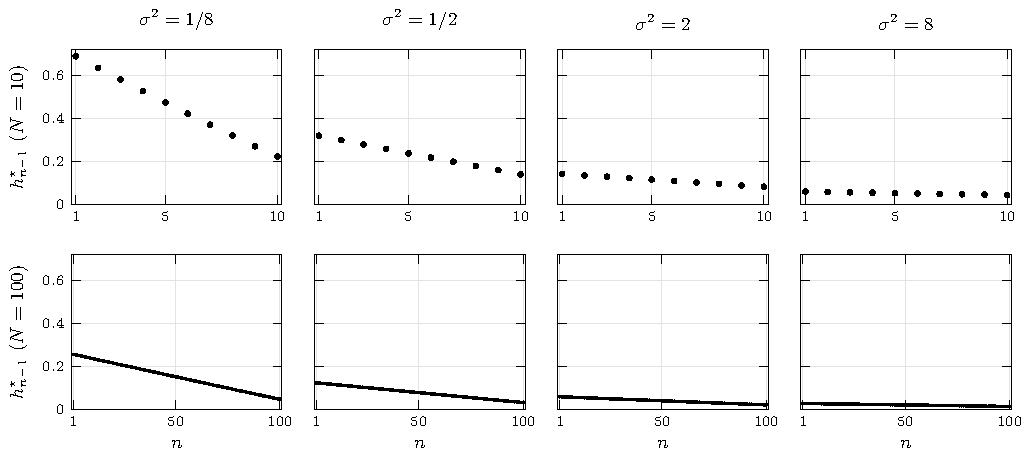
\includegraphics[width=\linewidth]{optimal_stepsizes.pdf}
    \caption{The exactly minimax optimal stepsize schedule $h^\star$ from~\eqref{eq:optimal-steps} for varied budgets $N$ and variances $\sigma^2$, fixing $L=D=1$. Asymptotically, this schedule behaves like the linear function~\eqref{eq:simple-asym-optimal-formula}.}
    \label{fig:stepsizes}
\end{figure}

\subsection{Related Work} \label{sec:related}


\section{Proof of Exact Lower Bound for any $h\in \mathbb{R}^N_+$} \label{sec:LB}

We construct our worst-case problem instance in dimension $d\geq N+1$ as follows:
Denote the $L$-smooth Huber function parameterized by a scalar $a\geq 0$ by
\begin{equation*}
    H_a(z) = \begin{cases}
        \frac{L}{2}|z|^2 & \text{if } |z|\leq a\\
        L a|z| - \frac{L}{2}a^2 & \text{otherwise}.
    \end{cases}
\end{equation*}
Note the degenerate case of $a=0$ has $H_0(z)=0$.
Let $e_0,e_1,\dots,e_N$ denote a collection of $N+1$ orthogonal unit vectors (which exist by our choice to work in dimension $d\geq N+1$). Define our worst-case problem instance's initialization $x_0 = De_0$.
Define our noise distributions at each iteration $n=1,\dots,N$ by the Rademacher distributions
\begin{equation} \label{eq:hard-distributions}
   \epsilon_{n-1} \sim P_{n-1}, \qquad \epsilon_{n-1} = \begin{cases}
        + \sigma e_n & \text{with probability }1/2\\
        - \sigma e_n & \text{with probability }1/2.
    \end{cases}
\end{equation}
Define our objective function by
\begin{equation} \label{eq:hard-function}
    f(x) = \sum_{i=0}^N H_{a_i}(\langle e_i, x\rangle)
\end{equation}
with $a_0 = \frac{D}{1+2 R_0}$ and $a_n = \frac{\sigma h_{n-1}}{
L\left(1+2R_n\right)
}$ for $n=1,\dots,N$.
The following lemma verifies this construction is indeed feasible for any choice of the parameters $L,D,\sigma^2 >0$.
\begin{lemma}
    The problem instance $\mathtt{p}$ defined by $x_0=De_0$, $f$ as in~\eqref{eq:hard-function}, and distributions $P_n$ as in~\eqref{eq:hard-distributions} is feasible, i.e., $\mathtt{p}\in\mathtt{P}(L,D,\sigma^2)$.
\end{lemma}
\begin{proof}
    First, observe that the function $f$ is minimized at the origin $x_\star=0$, having $f_\star=0$. Then, one can verify the needed initial condition as $\|x_0-x_\star\|=\|De_0\|=D$. The needed conditions for each noise distribution $P_n$ of zero-mean and $\sigma^2$-bounded variance follow directly from its definition.
    
    All that remains is to verify that $f$ is convex and $L$-smooth. A simple calculation can verify that the Huber function $H_a$ is convex and $L$-smooth for any $a\geq 0$. Since $f$ is a sum of these Huber functions, it inherits their convexity. Moreover, applying the chain rule, the gradient of $f$ is given by
    \begin{equation*}
        \nabla f(x) = \sum_{i=0}^N H_{a_i}'(\langle e_i,x\rangle)e_i.
    \end{equation*}
    Then $L$-smoothness of $f$ follows from $L$-smoothness of each Huber function as
    \begin{align*}
        \|\nabla f(x)-\nabla f(y)\|^2 &= \|\sum_{i=0}^N (H_{a_i}'(\langle e_i,x\rangle) - H_{a_i}'(\langle e_i,y\rangle))e_i\|^2\\
        &=\sum_{i=0}^N |H_{a_i}'(\langle e_i,x\rangle) - H_{a_i}'(\langle e_i,y\rangle)|^2\\
        &\leq L^2\sum_{i=0}^N |\langle e_i, x-y\rangle|^2\\
        &\leq L^2 \|x-y\|^2.
    \end{align*}
\end{proof}

\subsection{Proof of Lower Bound Half of Theorem~\ref{thm:main-rate}}
    Suppose one has applied SGD to this constructed problem instance. Below, we find that, for any realization of the noise sequence $\epsilon_n$, the claimed expected final iterate suboptimality is attained by the realized suboptimality. In particular, this constant final suboptimality establishes that the expectation over realizations is also exactly the claimed bound.

    Consider any sequence of signs $s_{n}\in\{\pm 1\}$ for $n=1,\dots,N$, providing a realization of errors from $P_{n-1}$ of $\epsilon_{n-1} = s_n \sigma e_n$. The key observation here is that the objective $f$ is separable over the coordinate directions $e_0,\dots,e_N$. So the progression of gradient descent in direction $e_i$ only depends on $\langle e_i, x_n\rangle$ (and no other directions). Thus we can analyze each direction separately.

    First consider the direction $e_0$. Each error $\epsilon_{n-1}$ is orthogonal to this direction, so SGD amounts to applying gradient descent deterministically to minimize $H_{a_0}(\langle e_0, x \rangle)$. This is a well-studied worst-case function for deterministic gradient descent~\cite{}. We claim inductively that every iterate $n=0,\dots,N$ has $\langle e_0, x_n\rangle \geq a_0$. At $n=0$, this is immediate as $D\geq a_0$. Inductively, this follows at some $n\geq 1$ as all prior iterations have derivative in direction $e_0$ of $H'_{a_0}(\langle e_0, x_{i}\rangle) = La_0$. So
    \begin{equation*}
        \langle e_0, x_n\rangle = \langle e_0, x_0\rangle - \sum_{i=0}^{n-1} h_i a_0 = a_0\left(1+2\sum_{i=0}^{N-1} h_i\right) - a_0 \sum_{i=0}^{n-1} h_i = a_0(1+R_0+R_n) \geq a_0
    \end{equation*}
    by noting $\langle e_0, x_0\rangle =D= a_0\left(1+2\sum_{i=0}^{N-1} h_i\right)$ from our choices of $x_0$ and $a_0$.
    
    In particular, the above calculation shows $\langle e_0, x_N\rangle = a_0(1+R_0)$. Hence, the final objective value on this first Huber function component is
    \begin{equation*}
        H_{a_0}(\langle e_0,x_N\rangle) = La_0| a_0(1+R_0)| - \frac{L}{2}a_0^2 = \frac{L}{2}a_0^2(1+2R_0) = \frac{LD^2}{2(1+2R_0)}.
    \end{equation*}

    The same calculations can be repeated on each component $e_1,\dots,e_N$. There, iterations $n=1,\dots,i-1$ have no effect on the $i$th component as $\langle e_i,x_n\rangle=0$. Then iteration $n=i$ will set $\langle e_i,x_i\rangle = -s_{i}\sigma h_{i-1}/L = -s_ia_i(1+2R_i)$. Thereafter, each iteration $n=i+1,\dots,N$ will perform deterministic gradient descent in this coordinate direction. Just as calculated above, gradient descent will always remain on the same (positive or negative) facet of the Huber function $H_{a_i}$, in particular having $\langle e_i,x_n\rangle = -s_ia_i(1+R_i+R_n)$. Continuing with the same calculation, this ensures the final iterate has 
    \begin{equation*}
        H_{a_i}(\langle e_i,x_N\rangle) = \frac{\sigma^2}{2L}\frac{h_{i-1}^2}{1+2 R_{i}},
    \end{equation*}
    regardless of the sampled sign $s_i$. Summing over each coordinate $e_0,\dots,e_{N}$ shows the claimed lower bound is attained on every realization of signs.



\section{Proof of Exact Convergence Guarantee for any $h\in [0,1.5]^N$} \label{sec:UB}

Some text introducing main ideas

\subsection{PEP-Style Convergence Proof}

The following are nonnegative or equal to zero for any problem \dots

This gives the primal PEP problem of\dots

If we find nonneg/psd multipliers such that the identity \dots holds, then we will have proven our target rate.

So our proof reduces to finding these.

In particular, we will use (define all values)

\begin{proposition}\label{prop:nonneg-mult}
    The scalars are nonnegative
\end{proposition}

\begin{proposition}\label{prop:psd-mult}
    The matrix is psd
\end{proposition}

\begin{proposition}\label{prop:identity}
    The identity holds
\end{proposition}

Once we prove these, the claimed rate and so all of our theorems and corollaries from the introduction follow.
We do this in parts in the following subsections, checking nonnegativeity and then agreement of each coefficient in the claimed affine identity.


\subsection{Proof of Nonnegativity (Proposition~\ref{prop:nonneg-mult})}

\subsection{Proof of Positive Semidefiniteness (Proposition~\ref{prop:psd-mult})}


\subsection{Useful Intermediate Identities and Lemmas}

\subsection{Verification of Main Identity (Proposition~\ref{prop:identity})}

\subsubsection{Verification of Constant Terms in Proposition~\ref{prop:identity}}


\subsubsection{Verification of \dots Terms in Proposition~\ref{prop:identity}}



\subsubsection{Verification of \dots Terms in Proposition~\ref{prop:identity}}

\subsubsection{Verification of \dots Terms in Proposition~\ref{prop:identity}}


\subsubsection{Verification of \dots Terms in Proposition~\ref{prop:identity}}

\subsubsection{Verification of \dots Terms in Proposition~\ref{prop:identity}}


\subsubsection{Verification of \dots Terms in Proposition~\ref{prop:identity}}

\subsubsection{Verification of \dots Terms in Proposition~\ref{prop:identity}}


\subsubsection{Verification of \dots Terms in Proposition~\ref{prop:identity}}

\subsubsection{Verification of \dots Terms in Proposition~\ref{prop:identity}}


\subsubsection{Verification of \dots Terms in Proposition~\ref{prop:identity}}


\section{Conclusion}



\section{Closed-formed expression of Multipliers}
The basic assumption: all entries in the stepsize schedule is between 0 and 1.5, that is:
\[h_i\in [0,1.5], \forall i = 0, 1, ....,N-1\] in other words, \[h^{(N)} \in [0, 1.5]^N\]\\
We study L-smooth and convex functions in $R^d$.



\todo[inline,color=cyan]{Define all needed nonnegative quantities here. Do not separate $Q_\star$ from $Q_i$'s. Allow $i\in\mathcal{I}=\{0,\dots,N,\star\}$ and $g_\star=0$. Aaron's paper is a good reference: \url{https://arxiv.org/pdf/2607.19240}}


\todo[inline,color=cyan]{State form of target proof $r - (f_N-f_\star) = \dots$.}


\todo[inline,color=cyan]{State all claimed multipliers below, not just $\lambda$.}

We consider the index set $\mathcal{I}=\{*,0,1,...,N\}$,
\[\forall i,j\in \mathcal{I}, Q_{i,j}:=f_i-f_j-\langle g_j,x_i-x_j\rangle -\frac{1}{2L}||g_i-g_j||^2\]
\[
V=
\left(
s,\,
g_0,\ldots,g_N,\,
\epsilon_0,\ldots,\epsilon_{N-1}
\right)^{T}.
\]
\[G=V^{\top}V\]
We set $L=1$\\
Next, we define a semidefinite programming problem to represent what we want to solve.
$\mathcal{R}(F,G):=R^2-||x_0-x_*||^2\quad \mathcal{Q}_{i,j}(F,G):= \forall i,j\in \mathcal{I}, Q_{i,j}:=Q_{i,j} \quad \forall i,j\in \mathcal{I}\quad \mathcal{S}_i(F,G):=\sigma_i^2-||\epsilon_i||^2 \quad $\\
An essential assumption is:\\
Class 1: \[\langle\epsilon_k, \epsilon_l \rangle = 0 \quad k \neq l\]
Class 2: \[\langle \epsilon_k, g_j\rangle = 0 \quad j\le k\]
Class 3: \[\langle \epsilon_k, x_j-x_* \rangle = 0 \quad j\le k\]
$F$ is a vector collecting function values from each iteration, that is:
\[F=[f_*, f_0,f_1, \ldots, f_N]^{\top} \in \mathbb{R}^{N+1}\]
{\color{red} Use $F=(f_0-f_\star, \dots, f_N-f_\star)$.}

Primal Problem\\

\begin{equation}
p^\star(h^{(N)}) = p_{\text{gram}}(h^{(N)}) = 
\left\{
\begin{aligned}
    \max_{F,G} \quad & (e_{N+2} - e_1)^{\top} F \\
    \text{s.t.} \quad & \mathcal{R}(F, G) \ge 0 \\
    & \mathcal{Q}_{i,j}(F, G) \ge 0 \quad \forall i, j \in \mathcal{I}_N \\
    & \mathcal{S}_i(F, G) \ge 0 \quad \forall i = 0, \dots, N \\
    & \mathcal{E}_{k,l}(F,G)=0  \quad \forall\, 0\le l<k\le N-1, \\
    & \mathcal{G}_{k,j}(F,G)=0  \quad \forall\, 0\le j\le k\le N-1, \\
    & \mathcal{X}_{k,0}(F,G)=0 \quad \forall\, k=0,\dots,N-1, \\
    & G \succeq 0.
\end{aligned}
\right.
\end{equation}
$\mathcal{E}_{k,l}(F,G)=0$ stands for $\langle\epsilon_k, \epsilon_l \rangle = 0$.\\
$\mathcal{G}_{k,j}(F,G)=0$ stands for $\langle\epsilon_k, g_j \rangle = 0$.\\
$\mathcal{X}_{k,0}(F,G)=0$ stands for $\langle\epsilon_k, x_0-x_\star \rangle = 0$.
Since each \(x_j-x_*\) is a linear combination of \(x_0-x_\star\), previous gradients, and previous noise terms, we reduced class 3 to $\mathcal{X}_{k,0}(F,G)=0.$
We define our multipliers below.\\
\[ \lambda_{\star,i} = \frac{h_i} {2\sum_{t=i}^{N-1}h_t} \prod_{k=0}^{i-1} \left(1-\frac{h_k}{2\sum_{t=k}^{N-1}h_t}\right),\qquad0\leq i\leq N-1,\]
\[ \lambda_{\star,N}= \prod_{k=0}^{N-1} \left( 1-\frac{h_k}{2\sum_{t=k}^{N-1}h_t} \right), \]
\[\lambda_{i,j}=\frac{h_i h_j}{4\left(\sum_{t=i}^{N-1}h_t\right) \left(\sum_{t=j}^{N-1}h_t\right)} \prod_{k=i+1}^{j-1} \left( 1-\frac{h_k}{2\sum_{t=k}^{N-1}h_t} \right), \qquad 0\leq i<j\leq N-1, \]
\[\lambda_{i,N}=\frac{h_i}{2\sum_{t=i}^{N-1}h_t}\prod_{k=i+1}^{N-1}
\left(1-\frac{h_k}{2\sum_{t=k}^{N-1}h_t}\right),\qquad 0\leq i\leq N-1,\]
The dual multiplier for distance constraint.
\[ \tau = \frac{1} {2\left(1+2\sum_{t=0}^{N-1}h_t\right)}, \]
Dual multipliers for noise constraint (from bounded variance assumption).
\[\eta_k=\frac{h_k^2} {2\left(1+2\sum_{t=k+1}^{N-1}h_t\right)}, \qquad 0\leq k\leq N-1, \]
Dual multipliers for $\mathcal{X}_{k,0}(F,G)=0 \quad \forall\, k=0,\dots,N-1 $
\[\xi_k= \frac{h_k} {1+2\sum_{t=k+1}^{N-1}h_t} \prod_{m=0}^{k} \left( 1-\frac{h_m}{2\sum_{t=m}^{N-1}h_t} \right), \qquad 0\leq k\leq N-1, \]
Dual multipliers for that noise in time $k$ should be orthogonal to all history information.(Affine constraints)\\
Dual multipliers for $\mathcal{G}_{k,j}(F,G)=0  \quad \forall\, 0\le j\le k\le N-1:$
\[ \mu_{i,k} = - \frac{h_k} {1+2\sum_{t=k+1}^{N-1}h_t} \left( h_i \frac{h_i}{2\sum_{t=i}^{N-1}h_t} \right) \prod_{m=i+1}^{k}
\left( 1-\frac{h_m}{2\sum_{t=m}^{N-1}h_t} \right), \qquad 0\leq i\leq k\leq N-1,\]
Dual multipliers for $\mathcal{E}_{k,l}(F,G)=0  \quad \forall\, 0\le l<k\le N-1$:
\[\nu_{\ell,k} = - \frac{h_\ell h_k} {1+2\sum_{t=k+1}^{N-1}h_t}
\prod_{m=\ell+1}^{k} \left( 1-\frac{h_m}{2\sum_{t=m}^{N-1}h_t} \right), \qquad 0\leq \ell<k\leq N-1. \]
Define \[\alpha_i=\frac{h_i}{2\sum_{t=i}^{N-1}h_t}\]
Then we define and give the closed form of dual multipliers of these nonnegative terms.\\
Type $1$: $\lambda_{*,i}$ will be:
\[\alpha_i\prod_{k=0}^{i-1}(1-\alpha_k)\]
For the brevity of notation, we define $\alpha_i = \frac{h_i}{2 S_i}$.\\
Type $2$ : For $0\le i< j\le N-1$, $\lambda_{i,j} = \alpha_i \alpha_j \prod_{k=i+1}^{j-1}(1-\alpha_k)$.\\
Type $3$: For $0\le i < j = N, \lambda_{i,j} = \alpha_i \prod_{k=i+1}^{N-1} (1-\alpha_k)$

We want to prove:
\[r-(f_N-f_*)=\tau \mathcal{R}+ \eta_i\mathcal{S}_i+ \sum_{i,j\in \mathcal{I}} \lambda_{i,j} \mathcal{Q}_{i,j}+\sum_{t\le k} \mu_{t,k} \mathcal{H}_k + \langle Z,G \rangle\]

\section{Verifying Nonnegativity and Positive Semidefiniteness}

\todo[inline,color=cyan]{Rename this section ``Verifying Nonnegativity and Positive Semidefiniteness''}

\todo[inline,color=cyan]{Stae as a proposition that all your multipliers are nonnegative/psd.}

\todo[inline,color=cyan]{Argue the scalar multipliers are each nonneg (short?)}

\todo[inline,color=cyan]{Then do the below reasoning to conclude Z is psd.}

\begin{proposition} All scalar multipliers are nonnegative.
\begin{proof}
 Clearly, $\tau$ and $\eta$ are non-negative.
 For all other multipliers, notice that $1-\frac{h_m}{\sum_{t\ge m}h_t}\ge 0$ and
 $h_i-\frac{h_i}{2\sum_{t\ge i} ht} \ge 0$
\end{proof}
    
\end{proposition}
Then our goal is to prove $\langle Z,G \rangle$ is nonnegative.\\
\subsection{definition of Z and prove it is PSD}
\[
Z=(K_NB_N)^{T}\widehat{W}_N(K_NB_N).
\] 
\[
B_N=\overline{B}_N+\widehat{B}_N,
\qquad
B_N\in\mathbb{R}^{(N+1)\times(2N+2)}.
\]

The columns of \(B_N\) are ordered according to
\[
V=
\left(
s,\,
g_0,\ldots,g_N,\,
\epsilon_0,\ldots,\epsilon_{N-1}
\right)^T.
\]

We define
\[
\overline{B}_N=
\begin{pmatrix}
1 & 0_{1\times(N+1)} & 0_{1\times N}\\
0_{N\times 1} & \Delta_N & 0_{N\times N}
\end{pmatrix},
\]
where
\[
\Delta_N=
\begin{pmatrix}
1&-1&0&\cdots&0&0\\
0&1&-1&\cdots&0&0\\
0&0&1&\ddots&0&0\\
\vdots&\vdots&\ddots&\ddots&\ddots&\vdots\\
0&0&0&\cdots&1&-1
\end{pmatrix}
\in\mathbb{R}^{N\times(N+1)}.
\]

Let
\[
H_N=
\operatorname{Diag}
\left(
\frac{h_0}{1+2S_1},
\frac{h_1}{1+2S_2},
\ldots,
\frac{h_{N-1}}{1+2S_N}
\right).
\]


\[
\widehat{B}_N=
\begin{pmatrix}
0 & -(1+2S_0)(1,0,\ldots,0) & 0_{1\times N}\\
0_{N\times1} & 0_{N\times(N+1)} & -H_N
\end{pmatrix}.
\]

Sum together
\[
B_N=
\begin{pmatrix}
1 & -T_0(1,0,\ldots,0) & 0_{1\times N}\\
0_{N\times1} & \Delta_N & -H_N
\end{pmatrix}.
\]

\[B_N=
\left(
\begin{array}{ccccccccccc}
1
&
-T_0 & 0 & 0 & \cdots & 0
&
0 & 0 & 0 & \cdots & 0
\\
0
&
1 & -1 & 0 & \cdots & 0
&
-\dfrac{h_0}{1+2S_1} & 0 & 0 & \cdots & 0
\\
0
&
0 & 1 & -1 & \ddots & \vdots
&
0 & -\dfrac{h_1}{1+2S_2} & 0 & \ddots & \vdots
\\
\vdots
&
\vdots & \ddots & \ddots & \ddots & 0
&
\vdots & \ddots & \ddots & \ddots & 0
\\
0
&
0 & \cdots & 0 & 1 & -1
&
0 & \cdots & 0 & 0
&-\dfrac{h_{N-1}}{1+2S_N}
\end{array}
\right),
\]
where the columns are ordered according to
\[
V=
\left(
s,\,
g_0,\ldots,g_N,\,
\epsilon_0,\ldots,\epsilon_{N-1}
\right)^{T}.
\]


\[
S_k:=\sum_{t=k}^{N-1}h_t,
\qquad
S_N:=0,
\qquad
T_k:=1+2S_k,
\qquad
T_N=1,
\]



The matrix \(K_N\in\mathbb{R}^{(N+1)\times(N+1)}\)
\[
(K_N)_{jk}
=
\begin{cases}
1,
& j=k=0,
\\(0.4em]
\displaystyle
2\prod_{m=j}^{k-1}(1-\alpha_m),
& 1\leq j\leq k\leq N,
\\(0.8em]
0,
& \text{otherwise}.
\end{cases}
\]


\[
K_N=
\begin{pmatrix}
1
&0
&0
&\cdots
&0
\\
0
&2
&2(1-\alpha_1)
&\cdots
&\displaystyle 2\prod_{m=1}^{N-1}(1-\alpha_m)
\\
0
&0
&2
&\cdots
&\displaystyle 2\prod_{m=2}^{N-1}(1-\alpha_m)
\\
\vdots
&\vdots
&\ddots
&\ddots
&\vdots
\\
0
&0
&\cdots
&2
&2(1-\alpha_{N-1})
\\
0
&0
&\cdots
&0
&2
\end{pmatrix}.
\]


\[
\widehat{W}_N
=
\Gamma_N
\oplus d_2
\oplus\cdots\oplus d_N,
\]
where
\[
\Gamma_N
=
\begin{pmatrix}
\displaystyle \frac{1}{2(1+2S_0)}
&
\displaystyle \frac{1-\alpha_0}{4}
\\(0.8em]
\displaystyle \frac{1-\alpha_0}{4}
&
\displaystyle \frac{1+2S_1}{8}
\end{pmatrix},
\]
and, for \(j=2,\ldots,N\),
\[
d_j
:=
\frac{(1+2S_j)-(1+2S_{j-1})(1-\alpha_{j-1})^{\,2}}{8}
=\frac{
h_{j-1}
\left[
(3-2h_{j-1})S_{j-1}+S_j
\right]
}{
32S_{j-1}^{\,2}
}\]





\[
\widehat{W}_N
=
\begin{pmatrix}
\Gamma_N
&
0
&
\cdots
&
0
\\
0
&
d_2
&&
0
\\
\vdots
&&
\ddots
&
\vdots
\\
0
&
0
&
\cdots
&
d_N
\end{pmatrix}.
\]
To prove that \(Z\) is PSD, it suffices to show that
\(\widehat{W}_N\) is PSD. Since
\[
\widehat{W}_N=\Gamma_N\oplus d_2\oplus\cdots\oplus d_N,
\]
it is enough to show that
$
\Gamma_N
$
is PSD and that \(d_j\geq 0\), for \(j=2,\ldots,N\).

\begin{lemma}
Suppose
\[
0<h_k\leq \frac{3}{2},\quad k=0,\ldots,N-1.
\]
\[d_j\ge 0\]

\end{lemma}

\begin{proof}
Since $h_{j-1}\in (0,\frac{3}{2}]$,
\[3-2h_{j-1}\ge 0\]
\[d_j=\frac{
h_{j-1}
\left[
(3-2h_{j-1})S_{j-1}+S_j
\right]
}{
32S_{j-1}^{\,2}
} \ge 0\]
\end{proof}
We find that $\Gamma_N$ can be decomposed as the sum of two rank-one matrices.\\
Define
\[\omega=\begin{pmatrix}
    1\\
    \frac{(1+2S_0)(1-\alpha_0)}{2}
\end{pmatrix}\]
\begin{lemma}[Positive semidefiniteness of the leading block]
The matrix
\[
\Gamma_N=
\frac{1}{2(1+2S_0)}
\omega\omega^\top
+
\frac{
(1+2S_1)-(1+2S_0)(1-\alpha_0)^2
}{8}
e_1e_1^\top.
\]
is PSD.
\end{lemma}

\begin{proof}
It suffices to show
\[
\frac{
(1+2S_1)-(1+2S_0)(1-\alpha_0)^2
}{8}\ge 0.
\]
Using
\[
S_1=S_0-h_0,
\qquad
\alpha_0=\frac{h_0}{2S_0},
\]
we have
\[
\begin{aligned}
&(1+2S_1)-(1+2S_0)(1-\alpha_0)^2\\
={}&
1+2S_0-2h_0
-(1+2S_0)(1-2\alpha_0+\alpha_0^2)\\
={}&
-2h_0+2\alpha_0(1+2S_0)
-\alpha_0^2(1+2S_0)\\
={}&
\alpha_0(2-h_0-\alpha_0).
\end{aligned}
\]
Since \(S_0\ge h_0\),
\[
0<\alpha_0=\frac{h_0}{2S_0}\le\frac12.
\]
Together with \(h_0\le\frac32\),
\[
2-h_0-\alpha_0\ge 0.
\]
Hence
\[
\frac{
(1+2S_1)-(1+2S_0)(1-\alpha_0)^2
}{8}\ge 0.
\]
\end{proof}

Combining Lemma $2.2$ and $2.3$,
\[
\widehat{W}_N
=\Gamma_N\oplus d_2\oplus\cdots\oplus d_N\succeq 0.
\]

\begin{theorem}
$\langle G,Z \rangle $ is nonnegative.
\end{theorem}

\begin{proof}
For any \(v\in\mathbb{R}^{2N+2}\), let
\[
y=K_NB_Nv.
\]
Then
\[
v^TZv
=v^T(K_NB_N)^T\widehat{W}_N(K_NB_N)v
=y^T\widehat{W}_Ny\geq 0.
\]
Therefore \(Z\succeq 0\).
And,
\[G= V^{\top}V\]
Hence, $\langle G,Z \rangle \ge 0$
\end{proof}

\section{Verifying Components}

\todo[inline,color=cyan]{State a prop that the needed equality holds for all your multlpiers}

\todo[inline,color=cyan]{Argue term-wise that coefficients match. The $f$ coefficients, the $\|x_0-x_\star\|^2$ coefficient, $\langle x_0-x_\star,g_i\rangle$, \dots}

\begin{lemma}
    \[\lambda_{*,j}+\sum_{p=0}^{i} \lambda_{p,j} = \alpha_j\prod_{m=i+1}^{j-1}(1-\alpha_m)\]
\end{lemma}

\begin{lemma}
    \[\alpha_i \prod_{k=j+1}^{i-1}(1-\alpha_k) =\prod_{k=j+1}^{i-1}(1-\alpha_k)-\prod_{k=j+1}^{i}(1-\alpha_k)\]
\end{lemma}
\begin{lemma}
\[\sum_{j=0}^{N}\lambda_{*,j}=1\]
\end{lemma}


{\color{cyan}

\subsection{Verification Constant Terms Agree}


We now verify that the multipliers defined in Section~5, together with the matrix
$Z$ defined in Section~6, satisfy the desired PEP identity.

\begin{proposition}
For every $N\ge 1$ and $h^{(N)}\in(0,1.5]^N$, let
$\tau$, $\eta_k$, $\lambda_{i,j}$, $\mu_{s,k}$,
$\mu_{g_i,k}$, $\mu_{\epsilon_\ell,k}$, and $Z$
be defined as in Sections~5 and~6. Then
\begin{equation}
\begin{aligned}
\frac{D^2}{2(1+2S_0)}+\sum_{k=0}^{N-1} \frac{h_k^2}{2(1+2S_{k+1})}-(f_N-f_\star)
={}&
\tau R(F,G)
+
\sum_{k=0}^{N-1}\eta_k S_k(F,G)
+
\sum_{i,j\in I}\lambda_{i,j}Q_{i,j}(F,G)
\\
&+
\sum_{t\le k}\mu_{t,k}H_k(F,G)
+
\langle Z,G\rangle,
\end{aligned}
\tag{7.1}
\end{equation}
\end{proposition}

We can verify the identity by verifying that each associated coefficient matches between the two sides.
Since 
\[\tau = \frac{1}{2(1+2S_0)}\]
\[\eta_k = \frac{h_k^2}{2(1+2S_{k+1})}\]
The coefficients of constant terms agree.


\subsection{Verification $f_i$ Coefficients Agree}
Next, we verify that the coefficients of the function values agree on the two sides of~(7.1).
Only the interpolation constraints $Q_{i,j}$ contain function-value terms.
Observe that, for the interpolation multipliers, only
\[\lambda_{\star,j}, \qquad j=0,\ldots,N,\]
and
\[\lambda_{i,j}, \qquad 0\le i<j\le N,\]
are nonzero.
\begin{lemma}
    \[\sum_{i,j\in \mathcal{I}} \lambda_{i,j} Q_{i,j}(F)=-(f_N-f_*)\]
\end{lemma}
\begin{proof}
Collecting the coefficient of each function value gives
\[\sum_{i,j\in I}\lambda_{i,j}(f_i-f_j)=\sum_{j=0}^{N-1}
\Big(\sum_{i=j+1}^{N}\lambda_{j,i}-\lambda_{\star,j}-\sum_{i=0}^{j-1}\lambda_{i,j}\Big)f_j-
\Big(\lambda_{\star,N}+\sum_{i=0}^{N-1}\lambda_{i,N}\Big)f_N
+\Big(\sum_{j=0}^{N}\lambda_{\star,j}\Big)f_\star.\]

By Lemma~7.1, for every $0\le j\le N-1$,
\[\lambda_{\star,j}+\sum_{i=0}^{j-1}\lambda_{i,j}=\alpha_j.\]

On the other hand, using the closed-form multipliers,
\[\sum_{i=j+1}^{N}\lambda_{j,i}=\alpha_j
\Big(\sum_{i=j+1}^{N-1}\alpha_i\prod_{k=j+1}^{i-1}(1-\alpha_k)+\prod_{k=j+1}^{N-1}(1-\alpha_k)\Big)\]
\[=\alpha_j\Big(\sum_{i=j+1}^{N-1}
\Big(\prod_{k=j+1}^{i-1}(1-\alpha_k)-\prod_{k=j+1}^{i}(1-\alpha_k)\Big)+\prod_{k=j+1}^{N-1}(1-\alpha_k)\Big)\]
\[=\alpha_j\Big(1+\sum_{i=j+1}^{N-2}\prod_{k=j+1}^{i}(1-\alpha_k)-\sum_{i=j+1}^{N-2}
\prod_{k=j+1}^{i}(1-\alpha_k)-\prod_{k=j+1}^{N-1}(1-\alpha_k)+\prod_{k=j+1}^{N-1}(1-\alpha_k)\Big)\]
\[=\alpha_j.\]

The second equality is from Lemma~7.2 and the third equality is from
$\prod_{k=j+1}^{j}(1-\alpha_k)=1$.

With Lemma~7.1, for every $j=0,\ldots,N-1$, the coefficient of $f_j$ is
\[\alpha_j-\alpha_j=0.\]

Since
\[\lambda_{\star,N}+\sum_{i=0}^{N-1}\lambda_{i,N}=1,\]
the coefficient of $f_N$ is $-1$.

The coefficient of $f_\star$ is
\[\sum_{j=0}^{N}\lambda_{\star,j}=1.\]
\end{proof}



\subsection{Verification $\|x_0-x_\star\|^2$ Coefficients Agree}
There are two sources for $\|x_0-x_\star\|^2$: $\tau R(F,G)$ and $\langle Z,G\rangle$, both of which are on the right hand side of $(7.1)$.
Since
\[R(F,G)=D^2-\|x_0-x_\star\|^2,\]
the coefficient from $\tau R(F,G)$ is $-\tau$.

Recall
\[Z=(K_NB_N)^T\widehat{W}_N(K_NB_N).\]
The column of $B_N$ corresponding to $x_0-x_\star$ is $e_1$, and $K_Ne_1=e_1$.
Hence, the coefficient of $\|x_0-x_\star\|^2$ in $\langle Z,G\rangle$ is
\[(\widehat{W}_N)_{1,1}=(\Gamma_N)_{1,1}=\tau.\]
Therefore, the coefficient of $\|x_0-x_\star\|^2$ on the right hand side of $(7.1)$ is
\[-\tau+\tau=0.\]



\subsection{Verification $\langle g_i, x_0-x_\star\rangle$ Coefficients Agree}
We consider coefficients of off-diagonal terms in the deterministic part. Two sources are
$\lambda_{*,i}Q_{*,i}$ and $\langle Z,G \rangle$. We need to show coefficients for $\langle g_i, x_0-x_* \rangle$ is equal to $-\lambda_{*,i}$
The column of $B_N$ corresponding to $x_0-x_\star$ is $e_1$, and \[K_Ne_1=e_1.\]
Since $\widehat{W}_N$ is block diagonal, only the first two entries of the column of $K_NB_N$ corresponding to $g_i$ contribute to $\langle g_i,x_0-x_\star\rangle$.
For $i=0$, the column of $B_N$ corresponding to $g_0$ is \[-(1+2S_0)e_1+e_2.\]
Hence,\[K_N(-(1+2S_0)e_1+e_2)=-(1+2S_0)e_1+2e_2.\]
Therefore,\[e_1^T\widehat{W}_N K_N(-(1+2S_0)e_1+e_2)=-\frac{1+2S_0}{2(1+2S_0)}+2\frac{1-\alpha_0}{4}\]
\[=-\frac{1}{2}+\frac{1-\alpha_0}{2}=-\frac{\alpha_0}{2}.\]
For $1\le i\le N-1$, the column of $B_N$ corresponding to $g_i$ is
\[-e_{i+1}+e_{i+2}.\]
The second entry of $K_N(-e_{i+1}+e_{i+2})$ is
\[-2\prod_{m=1}^{i-1}(1-\alpha_m)+2\prod_{m=1}^{i}(1-\alpha_m)\]
\[=-2\alpha_i\prod_{m=1}^{i-1}(1-\alpha_m).\]
Therefore,
\[e_1^T\widehat{W}_N K_N(-e_{i+1}+e_{i+2})=\frac{1-\alpha_0}{4}\left(-2\alpha_i\prod_{m=1}^{i-1}(1-\alpha_m)\right)\]
\[=-\frac{1}{2} \alpha_i\prod_{m=0}^{i-1}(1-\alpha_m) = -\frac{\lambda_{\star,i}}{2}.\]
Since $\langle g_i,x_0-x_\star\rangle$ is an off-diagonal Gram term, its coefficient
in $\langle Z,G\rangle$ is
\[-\lambda_{\star,i}.\]
For $i=N$, the column of $B_N$ corresponding to $g_N$ is
\[-e_{N+1}.\]
The second entry of $K_N(-e_{N+1})$ is
\[-2\prod_{m=1}^{N-1}(1-\alpha_m).\]
Therefore,
\[e_1^T\widehat{W}_N K_N(-e_{N+1})=\frac{1-\alpha_0}{4}\left(-2\prod_{m=1}^{N-1}(1-\alpha_m)
\right)\]
\[=-\frac{1}{2} \prod_{m=0}^{N-1}(1-\alpha_m) = -\frac{\lambda_{\star,N}}{2}.\]
Hence, the coefficient of $\langle g_N,x_0-x_\star\rangle$ in
$\langle Z,G\rangle$ is \[-\lambda_{\star,N}. \]
\begin{remark}
    Lemma form? And try to find a general way for the three types of multipliers.
\end{remark}


\subsection{Verification $\langle \epsilon_i, x_0-x_\star\rangle$ Coefficients Agree}
There are two sources for $\langle \epsilon_i,x_0-x_\star\rangle$:
the history orthogonality term with multiplier $\mu_{s,i}$ and$\langle Z,G\rangle$.
By definition,
\[\mu_{s,i}=\frac{h_i}{1+2S_{i+1}}\prod_{m=0}^{i}(1-\alpha_m).\]
Recall that
\[Z=(K_NB_N)^T\widehat{W}_N(K_NB_N).\]
The columns of $B_N$ corresponding to $x_0-x_\star$ and $\epsilon_i$ are
\[e_1\qquad\text{and}\qquad-\frac{h_i}{1+2S_{i+1}}e_{i+2}.\]
Since $K_Ne_1=e_1$, and the second entry of $K_Ne_{i+2}$ is
\[2\prod_{m=1}^{i}(1-\alpha_m),\]
we have\[e_1^TK_N^T\widehat{W}_NK_Ne_{i+2}=\frac{1-\alpha_0}{4}\cdot2\prod_{m=1}^{i}(1-\alpha_m)\]
\[=\frac{1}{2}\prod_{m=0}^{i}(1-\alpha_m).\]
Since $\langle \epsilon_i,x_0-x_\star\rangle$ is an off-diagonal Gram term,
its coefficient in $\langle Z,G\rangle$ is
\[-2\frac{h_i}{1+2S_{i+1}}e_1^TK_N^T\widehat{W}_NK_Ne_{i+2}\]
\[=-\frac{h_i}{1+2S_{i+1}}\prod_{m=0}^{i}(1-\alpha_m)\]
\[=-\mu_{s,i}.\]
Therefore, the coefficient of $\langle \epsilon_i,x_0-x_\star\rangle$ on the right hand side of $(7.1)$ is \[\mu_{s,i}-\mu_{s,i}=0.\]

\subsection{Verification $\langle g_i, g_j\rangle$ Coefficients Agree}
\subsubsection{$\|g_i\|^2$}
\begin{lemma}
    Sum of coefficients of $\|g_i\|^2$ from $\sum_{i,j \in \mathcal{I}}\lambda_{i,j} Q_{i,j}$ and $\langle Z,G \rangle$ equals to zero.
\end{lemma}
\begin{proof}
    For $0 \le i \le N-1$, the coefficient of $\|g_i\|^2$ is $- \frac{1}{2} (\lambda_{*,i} +\sum_{p=0}^{i-1} \lambda_{p,i} + \sum_{j=i+1}^N \lambda_{i,j})$\\
    By Lemma~7.1, \[\lambda_{\star,i}+\sum_{p=0}^{i-1}\lambda_{p,i}=\alpha_i.\]
    See section 7.2, we have \[\sum_{j=i+1}^{N} \lambda_{i,j} = \alpha_i\]
    Hence coefficient of $\|g_i\|^2$ from $\sum_{i,j \in \mathcal{I}}\lambda_{i,j} Q_{i,j}$
    is $-\alpha_i.$ for $0 \le i \le N-1.$\\
    Coefficient of $\|g_N\|^2$ from interpolation term is $-\frac{1}{2}.$, recall that $\alpha_N =1$ and we define $\prod_{a}^{b} (1-\alpha_a)=1.$
    For $i=0$, the column of $B_N$ corresponding to $g_0$ is
    \[-(1+2S_0)e_1+e_2.\]
    Hence,
    \[K_N(-(1+2S_0)e_1+e_2)=-(1+2S_0)e_1+2e_2.\]
    Therefore, the coefficient of $\|g_0\|^2$ from $\langle Z,G\rangle$ is
    \[\frac{1+2S_0}{2}-(1+2S_0)(1-\alpha_0)+\frac{1+2S_1}{2}\]
    \[=\frac{1+2S_1-(1+2S_0)}{2}+(1+2S_0)\alpha_0\]
    \[=-h_0+(1+2S_0)\alpha_0\]
    \[=-h_0+\alpha_0+h_0=\alpha_0.\]
    For $1\le i\le N-1$, the column of $B_N$ corresponding to $g_i$ is
    \[-e_{i+1}+e_{i+2}.\]
    By the definition of $K_N$,
    \[K_N(-e_{i+1}+e_{i+2})=-2\alpha_i\sum_{r=1}^{i}\prod_{m=r}^{i-1}(1-\alpha_m)e_{r+1}+ 2e_{i+2}.\]
    Hence, the coefficient of $\|g_i\|^2$ from $\langle Z,G\rangle$ is
    \[ 4\alpha_i^2 \left( \frac{1+2S_1}{8} \prod_{m=1}^{i-1}(1-\alpha_m)^2 + 
    \sum_{r=2}^{i} d_r \prod_{m=r}^{i-1}(1-\alpha_m)^2 \right) + 4d_{i+1}. \]
    By the definition of $d_r$, \[ \frac{1+2S_1}{8}\prod_{m=1}^{i-1}(1-\alpha_m)^2 +\sum_{r=2}^{i}d_r\prod_{m=r}^{i-1}(1-\alpha_m)^2 \]
\[ = \frac{1}{8} \left( (1+2S_1)\prod_{m=1}^{i-1}(1-\alpha_m)^2 + \sum_{r=2}^{i} 
\left( (1+2S_r)\prod_{m=r}^{i-1}(1-\alpha_m)^2 - (1+2S_{r-1})\prod_{m=r-1}^{i-1}(1-\alpha_m)^2 \right) \right) \]
\[ = \frac{1+2S_i}{8}, \]
where the last equality follows from telescoping.
Therefore, the coefficient of $\|g_i\|^2$ from $\langle Z,G\rangle$ is
\[\frac{\alpha_i^2(1+2S_i)}{2}+4d_{i+1}\]
\[=\frac{1}{2}
\left(
\alpha_i^2(1+2S_i)+(1+2S_{i+1})-(1+2S_i)(1-\alpha_i)^2
\right)\]
\[=\alpha_i(1+2S_i)-h_i=\alpha_i.\]
For $i=N$, the column of $B_N$ corresponding to $g_N$ is
\[-e_{N+1}.\]
Hence,
\[K_N(-e_{N+1})=-2\sum_{r=1}^{N}\prod_{m=r}^{N-1}(1-\alpha_m)e_{r+1}.\]
Therefore, the coefficient of $\|g_N\|^2$ from $\langle Z,G\rangle$ is
\[ 4\left(\frac{1+2S_1}{8}\prod_{m=1}^{N-1}(1-\alpha_m)^2+\sum_{r=2}^{N}d_r\prod_{m=r}^{N-1}(1-\alpha_m)^2\right).\]
By the same telescoping argument above,
\[4\left(\frac{1+2S_N}{8}\right)=\frac{1}{2},\] since $S_N=0$.
\end{proof}
\subsubsection{$\langle g_i, g_j \rangle \quad i<j$}
\begin{remark}
    One source of $\langle g_i, g_j \rangle$ is $x_p -x_j = \sum_{k=p}^{j-1}h_k(g_k+\epsilon_k)$, so if $p \le i$, it will contribute.\\
    In total, it is $-h_i(\lambda_{*,j}+ \sum_{p=0}^{i} \lambda_{p,j})=-h_i(\alpha_j \prod_{m=i+1}^{j-1}(1-\alpha_m))$
    Another source is from the norm square term: 
    \[-\frac{1}{2}\lambda_{i,j} \|g_i-g_j\|^2\]
    For $\langle Z,G \rangle$, we 
\end{remark}
\begin{lemma}
    Agrees
\end{lemma}
\begin{proof}
\[-h_i\alpha_j\prod_{m=i+1}^{j-1}(1-\alpha_m).\]
From\[-\frac{1}{2}\lambda_{i,j}\|g_i-g_j\|^2,\]
the coefficient of $\langle g_i,g_j\rangle$ is $\lambda_{i,j}$. Hence, the total coefficient from the interpolation terms is\[-h_i\alpha_j\prod_{m=i+1}^{j-1}(1-\alpha_m)+\lambda_{i,j}\]
\[=-h_i\alpha_j\prod_{m=i+1}^{j-1}(1-\alpha_m)+\alpha_i\alpha_j\prod_{m=i+1}^{j-1}(1-\alpha_m)\]
\[=-(h_i-\alpha_i)\alpha_j\prod_{m=i+1}^{j-1}(1-\alpha_m).\]
We then consider the coefficient from $\langle Z,G\rangle$.
Recall that
\[Z=(K_NB_N)^T\widehat{W}_N(K_NB_N).\]
From the calculation for $\langle \epsilon_i,\epsilon_j\rangle$, for
$0\le p\le q\le N-1$,\[e_{p+2}^T K_N^T\widehat{W}_NK_Ne_{q+2}=\frac{1+2S_{p+1}}{2}
\prod_{m=p+1}^{q}(1-\alpha_m).\]
Also, from the definition of $\Gamma_N$ and $K_N$,
\[e_1^T K_N^T\widehat{W}_NK_Ne_{q+2}=\frac{1}{2}\prod_{m=0}^{q}(1-\alpha_m).\]
First, consider $1\le i<j\le N-1$.
The columns of $B_N$ corresponding to $g_i$ and $g_j$ are
\[-e_{i+1}+e_{i+2}\qquad\text{and}\qquad-e_{j+1}+e_{j+2}.\]
Since $\langle g_i,g_j\rangle$ is an off-diagonal Gram term, its coefficient in
$\langle Z,G\rangle$ is
\[2(-e_{i+1}+e_{i+2})^T K_N^T\widehat{W}_NK_N (-e_{j+1}+e_{j+2})\]
\[=(1+2S_i)\prod_{m=i}^{j-1}(1-\alpha_m)-(1+2S_i)\prod_{m=i}^{j}(1-\alpha_m)\]
\[-(1+2S_{i+1})\prod_{m=i+1}^{j-1}(1-\alpha_m)+(1+2S_{i+1})\prod_{m=i+1}^{j}(1-\alpha_m)\]
\[=\alpha_j \prod_{m=i+1}^{j-1}(1-\alpha_m) \left((1+2S_i)(1-\alpha_i)-(1+2S_{i+1})\right).\]
Using $S_{i+1}=S_i-h_i$,
\[(1+2S_i)(1-\alpha_i)-(1+2S_{i+1})\]
\[=2h_i-\alpha_i(1+2S_i)\]
\[=2h_i-(h_i+\alpha_i)=h_i-\alpha_i.\]
Therefore, the coefficient from $\langle Z,G\rangle$ is
\[(h_i-\alpha_i)\alpha_j\prod_{m=i+1}^{j-1}(1-\alpha_m).\]
For $i=0$ and $1\le j\le N-1$, the columns of $B_N$ corresponding to
$g_0$ and $g_j$ are
\[-(1+2S_0)e_1+e_2\qquad\text{and}\qquad-e_{j+1}+e_{j+2}.\]
Hence, the coefficient from $\langle Z,G\rangle$ is
\[2(-(1+2S_0)e_1+e_2)^T K_N^T\widehat{W}_NK_N(-e_{j+1}+e_{j+2})\]
\[=(1+2S_0)\prod_{m=0}^{j-1}(1-\alpha_m)-(1+2S_0)\prod_{m=0}^{j}(1-\alpha_m)\]
\[-(1+2S_1)\prod_{m=1}^{j-1}(1-\alpha_m)+(1+2S_1)\prod_{m=1}^{j}(1-\alpha_m)\]
\[=\alpha_j\prod_{m=1}^{j-1}(1-\alpha_m)\left((1+2S_0)(1-\alpha_0)-(1+2S_1)\right)\]
\[=(h_0-\alpha_0)\alpha_j\prod_{m=1}^{j-1}(1-\alpha_m).\]
For $j=N$.
For $1\le i\le N-1$, the columns of $B_N$ corresponding to $g_i$ and $g_N$ are
\[-e_{i+1}+e_{i+2}\qquad\text{and}\qquad-e_{N+1}.\]
Hence, the coefficient from $\langle Z,G\rangle$ is
\[2(-e_{i+1}+e_{i+2})^TK_N^T\widehat{W}_NK_N(-e_{N+1})\]
\[=(1+2S_i)\prod_{m=i}^{N-1}(1-\alpha_m)-(1+2S_{i+1})\prod_{m=i+1}^{N-1}(1-\alpha_m)\]
\[=\left((1+2S_i)(1-\alpha_i)-(1+2S_{i+1})\right)\prod_{m=i+1}^{N-1}(1-\alpha_m)\]
\[=(h_i-\alpha_i)\prod_{m=i+1}^{N-1}(1-\alpha_m).\]
For $i=0$ and $j=N$,
\[2(-(1+2S_0)e_1+e_2)^T K_N^T\widehat{W}_NK_N(-e_{N+1})\]
\[=(1+2S_0)\prod_{m=0}^{N-1}(1-\alpha_m)-(1+2S_1)\prod_{m=1}^{N-1}(1-\alpha_m)\]
\[=(h_0-\alpha_0)\prod_{m=1}^{N-1}(1-\alpha_m).\]
Therefore, using $\alpha_N=1$, for every $0\le i<j\le N$, the coefficient of
$\langle g_i,g_j\rangle$ from $\langle Z,G\rangle$ is
\[(h_i-\alpha_i)\alpha_j\prod_{m=i+1}^{j-1}(1-\alpha_m).\]
\end{proof}

\subsection{Verification $\langle g_i, \epsilon_j\rangle$ Coefficients Agree}


\subsection{Verification $\langle \epsilon_i,\epsilon_j\rangle$ Coefficients Agree}
We consider the diagonal terms $\|\epsilon_i\|^2$ and the off-diagonal terms 
$\langle \epsilon_i,\epsilon_j\rangle$ separately.
\subsubsection{$\|\epsilon_i\|^2$}
There are two sources for $\|\epsilon_i\|^2$: $\eta_i S_i(F,G)$ and $\langle Z,G\rangle$.
Since
\[S_i(F,G)=\sigma_i^2-\|\epsilon_i\|^2,\]
the coefficient from $\eta_i S_i(F,G)$ is
\[-\eta_i=-\frac{h_i^2}{2(1+2S_{i+1})}.\]
Recall that
\[Z=(K_NB_N)^T\widehat{W}_N(K_NB_N).\]
The column of $B_N$ corresponding to $\epsilon_i$ is
\[-\frac{h_i}{1+2S_{i+1}}e_{i+2}.\]
Hence, the coefficient of $\|\epsilon_i\|^2$ in $\langle Z,G\rangle$ is
\[\frac{h_i^2}{(1+2S_{i+1})^2}e_{i+2}^T K_N^T\widehat{W}_N K_N e_{i+2}.\]
By the definition of $K_N$,
\[K_Ne_{i+2}=2\sum_{r=1}^{i+1}\prod_{m=r}^{i}(1-\alpha_m)e_{r+1}.\]
Therefore,
\[e_{i+2}^T K_N^T\widehat{W}_N K_Ne_{i+2}=4\left(\frac{1+2S_1}{8}\prod_{m=1}^{i}(1-\alpha_m)^2+\sum_{r=2}^{i+1} d_r\prod_{m=r}^{i}(1-\alpha_m)^2\right)\]
\[=\frac{1}{2}\left((1+2S_1)\prod_{m=1}^{i}(1-\alpha_m)^2+\sum_{r=2}^{i+1}\left(
(1+2S_r)-(1+2S_{r-1})(1-\alpha_{r-1})^2\right)\prod_{m=r}^{i}(1-\alpha_m)^2\right)\]
\[=\frac{1}{2}\left((1+2S_1)\prod_{m=1}^{i}(1-\alpha_m)^2+\sum_{r=2}^{i+1}(1+2S_r)\prod_{m=r}^{i}(1-\alpha_m)^2-\sum_{r=2}^{i+1}(1+2S_{r-1})\prod_{m=r-1}^{i}(1-\alpha_m)^2\right)\]
\[=\frac{1+2S_{i+1}}{2}.\]

Hence, the coefficient from $\langle Z,G\rangle$ is
\[\frac{h_i^2}{(1+2S_{i+1})^2}\frac{1+2S_{i+1}}{2}=\frac{h_i^2}{2(1+2S_{i+1})}
=\eta_i.\]
Therefore, the coefficient of $\|\epsilon_i\|^2$ on the right hand side of $(7.1)$ is
\[-\eta_i+\eta_i=0.\]

\subsubsection{$\langle \epsilon_i,\epsilon_j\rangle$}

Consider $0\le i<j\le N-1$.
There are two sources for $\langle \epsilon_i,\epsilon_j\rangle$: 
the history orthogonality term with multiplier $\mu_{\epsilon_i,j}$ 
and $\langle Z,G\rangle$.

The columns of $B_N$ corresponding to $\epsilon_i$ and $\epsilon_j$ are
\[-\frac{h_i}{1+2S_{i+1}}e_{i+2}\qquad\text{and}\qquad
-\frac{h_j}{1+2S_{j+1}}e_{j+2}.\]
Since $\langle \epsilon_i,\epsilon_j\rangle$ is an off-diagonal Gram term, 
its coefficient in $\langle Z,G\rangle$ is
\[2\frac{h_ih_j}{(1+2S_{i+1})(1+2S_{j+1})}e_{i+2}^T K_N^T\widehat{W}_N K_Ne_{j+2}.\]

Using the definition of $K_N$,
\[e_{i+2}^T K_N^T\widehat{W}_N K_Ne_{j+2}=4\left(\frac{1+2S_1}{8}\prod_{m=1}^{i}(1-\alpha_m)
\prod_{m=1}^{j}(1-\alpha_m)+\sum_{r=2}^{i+1} d_r\prod_{m=r}^{i}(1-\alpha_m)\prod_{m=r}^{j}(1-\alpha_m)\right)\]
\[=4\prod_{m=i+1}^{j}(1-\alpha_m)\left(\frac{1+2S_1}{8}\prod_{m=1}^{i}(1-\alpha_m)^2+
\sum_{r=2}^{i+1} d_r\prod_{m=r}^{i}(1-\alpha_m)^2\right)\]
\[=\frac{1+2S_{i+1}}{2}\prod_{m=i+1}^{j}(1-\alpha_m).\]

Hence, the coefficient from $\langle Z,G\rangle$ is
\[2\frac{h_ih_j}{(1+2S_{i+1})(1+2S_{j+1})}\frac{1+2S_{i+1}}{2}\prod_{m=i+1}^{j}(1-\alpha_m)
=\frac{h_ih_j}{1+2S_{j+1}}\prod_{m=i+1}^{j}(1-\alpha_m).\]

By the definition of $\mu_{\epsilon_i,j}$,
\[\mu_{\epsilon_i,j}=-\frac{h_ih_j}{1+2S_{j+1}}\prod_{m=i+1}^{j}(1-\alpha_m).\]
Therefore, the coefficient of $\langle \epsilon_i,\epsilon_j\rangle$ on the right hand side of $(7.1)$ is\[\mu_{\epsilon_i,j}-\mu_{\epsilon_i,j}=0.\]
}

\section{Section 3 renew}
\subsection{PEP-Style Convergence Proof}
Section~\ref{sec:LB} showed that the bound in Theorem~\ref{thm:main-rate} is attained by an explicit worst-case problem instance. We now prove the matching upper bound for every problem instance when $h\in[0,1.5]^N$. Denote the claimed rate by
\[r(h)=\frac{LD^2}{2(1+2R_0)}+\frac{\sigma^2}{2L} \sum_{k=0}^{N-1}
\frac{h_k^2}{1+2R_{k+1}}.\]
Following the framework of Performance Estimation Problems, we first
reduce~\eqref{eq:PEP} to a finite-dimensional optimization problem over
first-order information generated along the SGD trajectory. Let
\[ \mathcal I_N=\{\star,0,\ldots,N\}, \qquad f_i=f(x_i), \qquad g_i=\nabla f(x_i), \qquad g_\star=0. \]
By the smooth convex interpolation theorem of
Taylor, Hendrickx, and Glineur~\cite{taylor2017smooth}, any
$L$-smooth convex function satisfies, for every $i,j\in\mathcal I_N$,
\[ f_i-f_j -\langle g_j,x_i-x_j\rangle -\frac{1}{2L}\|g_i-g_j\|^2 \geq 0. \]
Define the interpolation quantities
\[\mathcal Q_{i,j}(F,G):=(f_i-f_\star)-(f_j-f_\star)-\langle g_j,x_i-x_j\rangle-\frac{1}{2L}\|g_i-g_j\|^2,\qquad i,j\in\mathcal I_N.\]
To express these quantities using finitely many variables, following the
stochastic PEP framework of Rubbens, Colla, and
Hendrickx~\cite{rubbens2025}, we use $F$ and $G$ to denote the
corresponding expected function-value and Gram variables. In particular,
collect the expected function-value gaps in
\[
F:=\mathbb E_\epsilon
\left[(f_0-f_\star,\ldots,f_N-f_\star)^\top\right]
\in\mathbb R^{N+1}.
\]
Let
\[
V=
\begin{bmatrix}
x_0-x_\star
&
g_0
&
\cdots
&
g_N
&
\epsilon_0
&
\cdots
&
\epsilon_{N-1}
\end{bmatrix},
\]
and define the expected Gram matrix
\[G:=\mathbb E_\epsilon[V^\top V]\succeq0.\]
To keep the notation light, we suppress expectation symbols from this
point onward: each function-value gap represented in $F$, and every
inner product or squared norm represented in $G$, is understood in this
expected sense. In particular, $\mathcal Q_{i,j}(F,G)$ denotes the
expectation of the interpolation quantity above. For example,
$\langle\epsilon_k,g_j\rangle$ denotes the corresponding entry
$\mathbb E_\epsilon[\langle\epsilon_k,g_j\rangle]$ of $G$.
The SGD recursion gives
\[x_j-x_\star=x_0-x_\star-\frac1L\sum_{t=0}^{j-1}
h_t(g_t+\epsilon_t),\qquad j=1,\ldots,N. \]
Hence every $x_j-x_\star$ is a linear combination of
$x_0-x_\star$, previous gradients, and previous noise terms, so no
additional iterate vectors are needed in the Gram representation.
After substituting these relations and taking expectations, each
$\mathcal Q_{i,j}(F,G)$ is affine in $F$ and $G$.
The initial-distance and bounded-variance assumptions similarly give
the nonnegative quantities
\[ \mathcal R(F,G) := D^2-\|x_0-x_\star\|^2 \geq0 \]
and \[ \mathcal S_k(F,G) := \sigma^2-\|\epsilon_k\|^2 \geq0, \qquad k=0,\ldots,N-1. \]
Moreover, following the stochastic PEP relaxation, the relevant moment consequences of independence and zero mean are encoded through orthogonality constraints with the history information. We write these relations as
\[ \mathcal E_{k,\ell}(F,G) := \langle\epsilon_k,\epsilon_\ell\rangle =0, \qquad 0\leq\ell<k\leq N-1, \]
\[ \mathcal G_{k,j}(F,G) := \langle\epsilon_k,g_j\rangle =0, \qquad 0\leq j\leq k\leq N-1, \]
and
\[ \mathcal X_{k,0}(F,G) := \langle\epsilon_k,x_0-x_\star\rangle =0, \qquad k=0,\ldots,N-1. \]
Together with the SGD recursion, these equalities also imply
$\langle\epsilon_k,x_j-x_\star\rangle=0$
for every $j\leq k$.
Consequently, every admissible problem instance in
$\mathtt P(L,D,\sigma^2)$ induces a feasible pair $(F,G)$ for the
following semidefinite relaxation:
\begin{equation}
\label{eq:gram-pep}
p_{\mathrm{gram}}(h,L,D,\sigma^2) =
\left\{ \begin{aligned}
\max_{F,G}\quad
    &e_{N+1}^\top F
\\
\mathrm{s.t.}\quad
    &\mathcal R(F,G)\geq0,
\\
    &\mathcal Q_{i,j}(F,G)\geq0,
        && i,j\in\mathcal I_N,
\\
    &\mathcal S_k(F,G)\geq0,
        && k=0,\ldots,N-1,
\\
    &\mathcal E_{k,\ell}(F,G)=0,
        &&0\leq\ell<k\leq N-1,
\\
    &\mathcal G_{k,j}(F,G)=0,
        &&0\leq j\leq k\leq N-1,
\\
    &\mathcal X_{k,0}(F,G)=0,
        &&k=0,\ldots,N-1,
\\
    &G\succeq0.
\end{aligned} \right.
\end{equation}
In particular, \[ \mathtt{PEP}(h,L,D,\sigma^2) \leq p_{\mathrm{gram}}(h,L,D,\sigma^2).\]
Thus it suffices to upper bound this SDP relaxation. We do not require
the relaxation itself to be exact; the matching construction in
Section~\ref{sec:LB} will ultimately show that our resulting upper bound
is tight in the regime of Theorem~\ref{thm:main-rate}.
By weak duality, we can formulate the dual problem of (9.1) and obtain the upper bound by solving it.
Our proof constructs explicit dual multipliers, given in closed form below, such that for all vectors $F$ and symmetric matrices $G$, \begin{equation}\label{eq:certificate-identity}
\begin{aligned}
r(h)-(f_N-f_\star) ={}& \tau \mathcal{R}(F,G) +\sum_{k=0}^{N-1}\eta_k \mathcal{S}_k(F,G) +\sum_{i,j\in\mathcal{I}_N}\lambda_{i,j}\mathcal{Q}_{i,j}(F,G) \\
&+ \sum_{k=0}^{N-1}\xi_k\mathcal{X}_{k,0}(F,G) +
\sum_{k=0}^{N-1}\sum_{j=0}^{k} \mu_{j,k}\mathcal{G}_{k,j}(F,G) \\
&+ \sum_{k=0}^{N-1}\sum_{\ell=0}^{k-1} \nu_{\ell,k}\mathcal{E}_{k,\ell}(F,G)
+ \langle Z,G\rangle .
\end{aligned}
\tag{3.1}
\end{equation}
The dual multipliers associated with the distance, variance, and interpolation constraints are nonnegative for every feasible problem, while the noise orthogonality terms are equal to zero. Thus, once the multipliers of the inequality constraints are shown to be nonnegative and $Z\succeq0$, identity~(3.1) immediately gives $f_N-f_\star\leq r(h)$.
The identity in~(3.1) is affine in the function values and Gram matrix entries. We therefore verify it by matching the coefficients on the two sides. We next specify the multipliers, and then verify their feasibility and the claimed identity.

For the remainder of the proof, we normalize $L=1$; the general result follows by rescaling the objective and stochastic gradients. We first consider $h\in(0,1.5]^N$, with the boundary cases obtained by continuity.
Recall\[R_k=\sum_{t=k}^{N-1}h_t,\qquad R_N=0,\] and define
\[ T_k:=1+2R_k, \qquad \alpha_k:=\frac{h_k}{2R_k}, \qquad k=0,\ldots,N-1. \]
For convenience, we additionally set
\[ T_N=1, \qquad \alpha_N:=1, \]
and interpret an empty product as one.
We now give the closed-form multipliers used in
\eqref{eq:certificate-identity}. The nonzero interpolation multipliers
are \[ \lambda_{\star,j} = \alpha_j \prod_{m=0}^{j-1}(1-\alpha_m), \qquad
j=0,\ldots,N, \]
and \[ \lambda_{i,j} = \alpha_i\alpha_j \prod_{m=i+1}^{j-1}(1-\alpha_m),
\qquad 0\leq i<j\leq N. \]
All remaining interpolation multipliers are set to zero.
The multiplier associated with the initial distance constraint is
\[ \tau=\frac{1}{2T_0}, \]
and the multipliers associated with the variance constraints are
\[ \eta_k=\frac{h_k^2}{2T_{k+1}}, \qquad k=0,\ldots,N-1. \]

For the affine orthogonality constraints, define
\[ \xi_k = \frac{h_k}{T_{k+1}} \prod_{m=0}^{k}(1-\alpha_m),
\qquad k=0,\ldots,N-1, \]
\[ \mu_{j,k} = - \frac{h_k}{T_{k+1}} (h_j-\alpha_j) \prod_{m=j+1}^{k}(1-\alpha_m), \qquad 0\leq j\leq k\leq N-1, \]
and \[ \nu_{\ell,k} = - \frac{h_\ell h_k}{T_{k+1}} \prod_{m=\ell+1}^{k}(1-\alpha_m), \qquad 0\leq\ell<k\leq N-1. \]
It remains to define the positive semidefinite multiplier $Z$. Let
\[H_N = \operatorname{Diag} \left( \frac{h_0}{T_1}, \frac{h_1}{T_2},
\ldots, \frac{h_{N-1}}{T_N} \right) \]
and let \[ \Delta_N =
\begin{pmatrix}
1&-1&0&\cdots&0\\
0&1&-1&\ddots&\vdots\\
\vdots&\ddots&\ddots&\ddots&0\\
0&\cdots&0&1&-1
\end{pmatrix}
\in\mathbb R^{N\times(N+1)}. \]
Define \[ B_N =
\begin{pmatrix}
1 & -T_0 e_1^\top & 0_{1\times N}\\
0_{N\times1} & \Delta_N & -H_N
\end{pmatrix}, \]
where $e_1$ denotes the first standard basis vector of
$\mathbb R^{N+1}$.
Next, define $K_N\in\mathbb R^{(N+1)\times(N+1)}$ by
\[ (K_N)_{jk} = \begin{cases} 1, &j=k=0, \\[0.4em]
\displaystyle 2\prod_{m=j}^{k-1}(1-\alpha_m),
&1\leq j\leq k\leq N, \\[0.6em] 0,
&\text{otherwise}. \end{cases} \]
Finally, let
\[\widehat W_N = \Gamma_N\oplus d_2\oplus\cdots\oplus d_N, \]
where
\[ \Gamma_N = \begin{pmatrix} \displaystyle\frac{1}{2T_0} & \displaystyle\frac{1-\alpha_0}{4} \\[0.7em]
\displaystyle\frac{1-\alpha_0}{4}
& \displaystyle\frac{T_1}{8}
\end{pmatrix} \]
and, for $j=2,\ldots,N$,
\[ d_j := \frac{ T_j-T_{j-1}(1-\alpha_{j-1})^2 }{8}. \]
The Gram multiplier in \eqref{eq:certificate-identity} is
\[ Z = (K_NB_N)^\top \widehat W_N (K_NB_N). \]
These formulas completely specify the certificate in \eqref{eq:certificate-identity}. The proof reduces to the following three propositions.
\begin{proposition}\label{prop:nonnegative-multipliers}
The multipliers associated with the inequality constraints satisfy $\tau\ge0$, $\eta_k\ge0$, $\lambda_{\star,j}\ge0$, and $\lambda_{i,j}\ge0$.
\end{proposition}
\begin{proposition}\label{prop:psd-gram-multiplier}
For $h\in (0,3/2]^N$, the Gram multiplier $Z$ is positive semidefinite.
\end{proposition}
\begin{proposition}\label{prop:certificate-identity}
For any $h\in(0,3/2]^N$, the multipliers defined above satisfy the certificate identity~\eqref{eq:certificate-identity} for every $F\in\mathbb R^{N+1}$ and $G\in \mathbb{S}^{2N+2}$.
\end{proposition}
\subsection{Proof of Nonnegativity (Proposition~\ref{prop:nonnegative-multipliers})}
\begin{proof}
Since $R_k\ge h_k>0$, we have $0<\alpha_k=h_k/(2R_k)\le1/2$ for $k=0,\ldots,N-1$. Hence every factor in the nonzero interpolation multipliers is nonnegative, so all $\lambda_{\star,j}$ and $\lambda_{i,j}$ are nonnegative; the nonnegativity of $\tau$ and $\eta_k$ is immediate from their definitions.
\end{proof}

\subsection{Proof of Positive Semidefiniteness (Proposition~\ref{prop:psd-gram-multiplier})}
\begin{proof}
Using the factorization
\[Z=(K_NB_N)^\top\widehat W_N(K_NB_N),\]
it is enough to prove that $\widehat W_N\succeq0$. Since
\[\widehat W_N=\Gamma_N\oplus d_2\oplus\cdots\oplus d_N,\]
this reduces to showing that $d_j\ge0$ for $j=2,\ldots,N$ and
$\Gamma_N\succeq0$.
For $j=2,\ldots,N$, direct simplification gives
\[d_j= \frac{h_{j-1}\big[(3-2h_{j-1})R_{j-1}+R_j\big]} {32R_{j-1}^2}. \]
Since $0<h_{j-1}\le3/2$ and $R_j\ge0$, we have $d_j\ge0$.
For the leading block, define
\[ \omega=
\begin{pmatrix} 1
\\ T_0(1-\alpha_0)/2 
\end{pmatrix}. \]
Then
\[ \Gamma_N =
\frac{1}{2T_0}\omega\omega^\top + \frac{T_1-T_0(1-\alpha_0)^2}{8}e_2e_2^\top, \]
where $e_2=(0,1)^\top$.
The first term is positive semidefinite, while
\[ T_1-T_0(1-\alpha_0)^2 = \alpha_0(2-h_0-\alpha_0). \]
Since $0<\alpha_0\le1/2$ and $h_0\le3/2$,
\[ 2-h_0-\alpha_0\ge0. \]
Hence $\Gamma_N\succeq0$, and therefore $\widehat W_N\succeq0$.
Consequently,
\[ Z=(K_NB_N)^\top\widehat W_N(K_NB_N)\succeq0. \]
\end{proof}
\subsection{Useful Intermediate Identities and Lemmas}
The following identities will be used to verify (3.1) by coefficient matching.
\begin{lemma}\label{lem:lambda-partial-sum}
For $0\le i<j\le N$,
\[ \lambda_{\star,j}+\sum_{p=0}^{i}\lambda_{p,j} =\alpha_j\prod_{m=i+1}^{j-1}(1-\alpha_m). \]
\end{lemma}
\begin{proof}
By the definitions of the interpolation multipliers,
\[\lambda_{\star,j}+\sum_{p=0}^{i}\lambda_{p,j}
=\alpha_j\prod_{m=0}^{j-1}(1-\alpha_m)
+\alpha_j\sum_{p=0}^{i}\alpha_p\prod_{m=p+1}^{j-1}(1-\alpha_m).\]
For each $p$, factoring out the common product gives
\[\begin{aligned}
&\prod_{m=p+1}^{j-1}(1-\alpha_m)-\prod_{m=p}^{j-1}(1-\alpha_m)\\
&=[1-(1-\alpha_p)]\prod_{m=p+1}^{j-1}(1-\alpha_m)
=\alpha_p\prod_{m=p+1}^{j-1}(1-\alpha_m).
\end{aligned} \]
Hence the sum telescopes as
\[\sum_{p=0}^{i}\alpha_p\prod_{m=p+1}^{j-1}(1-\alpha_m)
=\prod_{m=i+1}^{j-1}(1-\alpha_m)-\prod_{m=0}^{j-1}(1-\alpha_m).\]
Substituting this above gives
\[\lambda_{\star,j}+\sum_{p=0}^{i}\lambda_{p,j} =\alpha_j\prod_{m=i+1}^{j-1}(1-\alpha_m). \]
\end{proof}
\begin{lemma}\label{lem:lambda-outgoing-sum}
For $0\le i\le N-1$,
\[\sum_{j=i+1}^{N}\lambda_{i,j}=\alpha_i.\]
\end{lemma}
\begin{proof}
By the definitions of the interpolation multipliers and $\alpha_N=1$,
\[ \sum_{j=i+1}^{N}\lambda_{i,j}
=\alpha_i\left(\sum_{j=i+1}^{N-1}\alpha_j\prod_{m=i+1}^{j-1}(1-\alpha_m)
+\prod_{m=i+1}^{N-1}(1-\alpha_m)\right). \]
For each $j=i+1,\ldots,N-1$,
\[ \alpha_j\prod_{m=i+1}^{j-1}(1-\alpha_m)
=\prod_{m=i+1}^{j-1}(1-\alpha_m)-\prod_{m=i+1}^{j}(1-\alpha_m). \]
Recall that the empty product is defined to be $1$. Using the telescoping sum, \[ \sum_{j=i+1}^{N-1}\alpha_j\prod_{m=i+1}^{j-1}(1-\alpha_m)
=1-\prod_{m=i+1}^{N-1}(1-\alpha_m). \]
Substituting this above gives
\[ \sum_{j=i+1}^{N}\lambda_{i,j}=\alpha_i. \]
\end{proof}
\begin{lemma}\label{lem:gram-kernel}
Let $M_N:=K_N^\top\widehat W_NK_N$. Then
\[(M_N)_{1,1}=\frac{1}{2T_0},\]
\[(M_N)_{1,q+2}=\frac12\prod_{m=0}^{q}(1-\alpha_m), \qquad 0\le q\le N-1,\]
and
\[(M_N)_{p+2,q+2} =\frac{T_{p+1}}2\prod_{m=p+1}^{q}(1-\alpha_m),\qquad 0\le p\le q\le N-1.\]
\end{lemma}
\begin{proof}
Since $K_Ne_1=e_1$, the first identity follows directly from the leading entry of $\widehat W_N$.
For the second identity, the definition of $K_N$ gives
\[K_Ne_{q+2}=2\sum_{r=1}^{q+1}\prod_{m=r}^{q}(1-\alpha_m)e_{r+1}. \]
Since $K_Ne_{q+2}$ has no $e_1$ component, only the $(1,2)$ entry of the leading block $\Gamma_N$ contributes. Hence
\[(M_N)_{1,q+2}=\frac{1-\alpha_0}{4}\,2\prod_{m=1}^{q}(1-\alpha_m)
=\frac12\prod_{m=0}^{q}(1-\alpha_m). \]
For the third identity, using the same expression for the columns of $K_N$ and factoring out the common product gives
\[\begin{aligned} (M_N)_{p+2,q+2}=4\prod_{m=p+1}^{q}(1-\alpha_m)\Bigg( &\frac{T_1}{8}\prod_{m=1}^{p}(1-\alpha_m)^2 +\sum_{r=2}^{p+1}d_r\prod_{m=r}^{p}(1-\alpha_m)^2 \Bigg). \end{aligned} \]
By the definition of $d_r$, the expression in parentheses becomes
\[\frac18\left( T_1\prod_{m=1}^{p}(1-\alpha_m)^2 +\sum_{r=2}^{p+1}
\left[T_r\prod_{m=r}^{p}(1-\alpha_m)^2 -T_{r-1}\prod_{m=r-1}^{p}(1-\alpha_m)^2\right] \right). \]
The consecutive terms cancel, leaving $T_{p+1}/8$. Therefore
\[(M_N)_{p+2,q+2}
=\frac{T_{p+1}}2\prod_{m=p+1}^{q}(1-\alpha_m). \]
\end{proof}
\begin{lemma}\label{lem:T-alpha}
For $k=0,\ldots,N-1$,
\[ T_k\alpha_k=h_k+\alpha_k, \qquad T_k(1-\alpha_k)-T_{k+1}=h_k-\alpha_k.
\]
\end{lemma}
\begin{proof}
By the definitions of $T_k$ and $\alpha_k$,
\[ T_k\alpha_k=(1+2R_k)\frac{h_k}{2R_k}=h_k+\alpha_k. \]
Moreover, since $R_{k+1}=R_k-h_k$, we have $T_{k+1}=T_k-2h_k$. Therefore,
\[ \begin{aligned}
T_k(1-\alpha_k)-T_{k+1}
&=T_k-T_k\alpha_k-(T_k-2h_k)\\
&=2h_k-(h_k+\alpha_k)
=h_k-\alpha_k.
\end{aligned} \]
\end{proof}

\subsection{Verification of Main Identity (Proposition~\ref{prop:certificate-identity})}
Observe that (3.1) is affine in $F$ and $G$. We therefore prove Proposition~\ref{prop:certificate-identity} by matching the coefficients on the two sides: it suffices to verify agreement of the constant and function-value terms, together with the coefficients of all squared-norm and inner-product terms represented in $G$.
\subsubsection{Verification of Constant Terms in Proposition~\ref{prop:certificate-identity}}
The constant terms agree, since their correspondence amounts to
\[\tau D^2+\sum_{k=0}^{N-1}\eta_k\sigma^2= \frac{D^2}{2T_0}
+\frac{\sigma^2}{2}\sum_{k=0}^{N-1}\frac{h_k^2}{T_{k+1}}, \]
which follows immediately from
\[ \tau=\frac{1}{2T_0}, \qquad \eta_k=\frac{h_k^2}{2T_{k+1}}. \]
\subsubsection{Verification of Function-Value Terms in Proposition~\ref{prop:certificate-identity}}
Only the interpolation constraints depend on $F$. For $j=0,\ldots,N-1$, the coefficient of $f_j-f_\star$ is
\[\sum_{i=j+1}^{N}\lambda_{j,i}-\lambda_{\star,j}-\sum_{i=0}^{j-1}\lambda_{i,j}.\]
For $j\ge1$, Lemma~\ref{lem:lambda-partial-sum} with $i=j-1$ gives
\[\lambda_{\star,j}+\sum_{i=0}^{j-1}\lambda_{i,j}=\alpha_j.\]
For $j=0$, the same equality follows directly from $\lambda_{\star,0}=\alpha_0$. By Lemma~\ref{lem:lambda-outgoing-sum},
\[ \sum_{i=j+1}^{N}\lambda_{j,i}=\alpha_j.\]
Hence the coefficient of $f_j-f_\star$ is zero for every $j=0,\ldots,N-1$.
For $j=N$, Lemma~\ref{lem:lambda-partial-sum} with $i=N-1$, together with $\alpha_N=1$, gives
\[\lambda_{\star,N}+\sum_{i=0}^{N-1}\lambda_{i,N}=1.\]
Thus the coefficient of $f_N-f_\star$ is $-1$, and the function-value terms reduce to
\[-(f_N-f_\star),\] as required.
\subsubsection{Verification of $\|x_0-x_\star\|^2$ in Proposition~\ref{prop:certificate-identity}}
We next consider the coefficient of $\|x_0-x_\star\|^2$. It receives contributions from $\tau\mathcal R(F,G)$ and $\langle Z,G\rangle$. Since the column of $B_N$ corresponding to $x_0-x_\star$ is $e_1$, Lemma~\ref{lem:gram-kernel} gives
\[-\tau+(M_N)_{1,1}=-\frac{1}{2T_0}+\frac{1}{2T_0}=0.\]
\subsubsection{Verification of $\langle g_i,x_0-x_\star\rangle$ in Proposition~\ref{prop:certificate-identity}}
Next consider $\langle g_i,x_0-x_\star\rangle$. The interpolation term $\lambda_{\star,i}\mathcal Q_{\star,i}$ contributes $\lambda_{\star,i}$, while the remaining contribution comes from $\langle Z,G\rangle$. The columns of $B_N$ corresponding to $g_i$ are
\[-T_0e_1+e_2\quad(i=0),\qquad -e_{i+1}+e_{i+2}\quad(1\le i\le N-1),\qquad
-e_{N+1}\quad(i=N). \]
Using Lemma~\ref{lem:gram-kernel}, the contribution from $\langle Z,G\rangle$ is \[ \begin{cases}
2\left[-T_0(M_N)_{1,1}+(M_N)_{1,2}\right]=-\alpha_0,&i=0,\\
2\left[-(M_N)_{1,i+1}+(M_N)_{1,i+2}\right]
=-\alpha_i\displaystyle\prod_{m=0}^{i-1}(1-\alpha_m),&1\le i\le N-1,\\
-2(M_N)_{1,N+1}
=-\displaystyle\prod_{m=0}^{N-1}(1-\alpha_m),&i=N,
\end{cases} \]
which equals $-\lambda_{\star,i}$ in each case. Hence the coefficient of $\langle g_i,x_0-x_\star\rangle$ is zero.
\subsubsection{Verification of $\langle\epsilon_k,x_0-x_\star\rangle$ in Proposition~\ref{prop:certificate-identity}}
We next consider $\langle\epsilon_k,x_0-x_\star\rangle$. Its coefficient receives contributions from $\xi_k\mathcal X_{k,0}(F,G)$ and $\langle Z,G\rangle$. The column of $B_N$ corresponding to $\epsilon_k$ is
\[ -\frac{h_k}{T_{k+1}}e_{k+2}. \]
Therefore, by Lemma~\ref{lem:gram-kernel}, the contribution from $\langle Z,G\rangle$ is
\[-\frac{2h_k}{T_{k+1}}(M_N)_{1,k+2} =-\frac{h_k}{T_{k+1}}\prod_{m=0}^{k}(1-\alpha_m) =-\xi_k.\]
Hence the coefficient of $\langle\epsilon_k,x_0-x_\star\rangle$ is zero.
\subsubsection{Verification of $\|\epsilon_k\|^2$ in Proposition~\ref{prop:certificate-identity}}
For $\|\epsilon_k\|^2$, the two contributions come from $\eta_k\mathcal S_k(F,G)$ and $\langle Z,G\rangle$. Using the same column of $B_N$ and Lemma~\ref{lem:gram-kernel},
\[ \frac{h_k^2}{T_{k+1}^2}(M_N)_{k+2,k+2} =\frac{h_k^2}{2T_{k+1}}
=\eta_k. \]
Thus the coefficient of $\|\epsilon_k\|^2$ is
\[ -\eta_k+\eta_k=0. \]
\subsubsection{Verification of $\langle\epsilon_\ell,\epsilon_k\rangle$ in Proposition~\ref{prop:certificate-identity}}
Finally, for $0\le\ell<k\le N-1$, the coefficient of $\langle\epsilon_\ell,\epsilon_k\rangle$ receives contributions from $\nu_{\ell,k}\mathcal E_{k,\ell}(F,G)$ and $\langle Z,G\rangle$. By Lemma~\ref{lem:gram-kernel},
\[ \frac{2h_\ell h_k}{T_{\ell+1}T_{k+1}} (M_N)_{\ell+2,k+2}
= \frac{h_\ell h_k}{T_{k+1}} \prod_{m=\ell+1}^{k}(1-\alpha_m) =-\nu_{\ell,k}. \]
Hence the coefficient of $\langle\epsilon_\ell,\epsilon_k\rangle$ is zero.

\subsubsection{Verification of $\|g_i\|^2$ in Proposition~\ref{prop:certificate-identity}}
We next consider the coefficient of $\|g_i\|^2$. For $0\le i\le N-1$, the interpolation terms contribute
\[
-\frac12\left(\lambda_{\star,i}+\sum_{p=0}^{i-1}\lambda_{p,i}+\sum_{j=i+1}^{N}\lambda_{i,j}\right)=-\alpha_i,
\]
where Lemmas~\ref{lem:lambda-partial-sum} and~\ref{lem:lambda-outgoing-sum} are used, with the case $i=0$ following directly from $\lambda_{\star,0}=\alpha_0$. For $i=N$, Lemma~\ref{lem:lambda-partial-sum} with $i=N-1$ and $\alpha_N=1$ gives
\[
-\frac12\left(\lambda_{\star,N}+\sum_{p=0}^{N-1}\lambda_{p,N}\right)=-\frac12.
\]
It remains to compute the contribution from $\langle Z,G\rangle$. Using the columns of $B_N$ corresponding to $g_i$ and Lemma~\ref{lem:gram-kernel}, this contribution is
\[
\begin{cases}
T_0^2(M_N)_{1,1}-2T_0(M_N)_{1,2}+(M_N)_{2,2}
=-h_0+T_0\alpha_0=\alpha_0,&i=0,\\[0.4em]
(M_N)_{i+1,i+1}-2(M_N)_{i+1,i+2}+(M_N)_{i+2,i+2}
=-h_i+T_i\alpha_i=\alpha_i,&1\le i\le N-1,\\[0.4em]
(M_N)_{N+1,N+1}=\dfrac12,&i=N,
\end{cases}\]
where we used $T_{i+1}=T_i-2h_i$ and Lemma~\ref{lem:T-alpha}. Hence the coefficient of $\|g_i\|^2$ is zero for every $i=0,\ldots,N$.
\subsubsection{Verification of $\langle g_i,g_j\rangle$ in Proposition~\ref{prop:certificate-identity}}
Consider $0\le i<j\le N$. From the interpolation constraints, the terms $-\langle g_j,x_p-x_j\rangle$ contribute whenever $p=\star$ or $0\le p\le i$, while the squared-gradient term in $\mathcal Q_{i,j}$ contributes $\lambda_{i,j}$. Hence, by Lemma~\ref{lem:lambda-partial-sum},
\[\begin{aligned}
&-h_i\left(\lambda_{\star,j}+\sum_{p=0}^{i}\lambda_{p,j}\right)+\lambda_{i,j}\\
&=-(h_i-\alpha_i)\alpha_j\prod_{m=i+1}^{j-1}(1-\alpha_m).
\end{aligned}\]
We next compute the contribution from $\langle Z,G\rangle$. For $1\le i<j\le N-1$, Lemma~\ref{lem:gram-kernel} gives
\[ \begin{aligned}
&2(-e_{i+1}+e_{i+2})^\top M_N(-e_{j+1}+e_{j+2})\\
={}&T_i\prod_{m=i}^{j-1}(1-\alpha_m)-T_i\prod_{m=i}^{j}(1-\alpha_m)
-T_{i+1}\prod_{m=i+1}^{j-1}(1-\alpha_m)+T_{i+1}\prod_{m=i+1}^{j}(1-\alpha_m)\\
={}&\alpha_j\prod_{m=i+1}^{j-1}(1-\alpha_m)\left[T_i(1-\alpha_i)-T_{i+1}\right]\\
={}&(h_i-\alpha_i)\alpha_j\prod_{m=i+1}^{j-1}(1-\alpha_m),
\end{aligned} \]
where the last equality follows from Lemma~\ref{lem:T-alpha}. The boundary cases follow from the corresponding columns of $B_N$:
\[ \begin{aligned}
2(-T_0e_1+e_2)^\top M_N(-e_{j+1}+e_{j+2})
&=(h_0-\alpha_0)\alpha_j\prod_{m=1}^{j-1}(1-\alpha_m), &&1\le j\le N-1,\\
2(-e_{i+1}+e_{i+2})^\top M_N(-e_{N+1})
&=(h_i-\alpha_i)\prod_{m=i+1}^{N-1}(1-\alpha_m), &&1\le i\le N-1,\\
2(-T_0e_1+e_2)^\top M_N(-e_{N+1})
&=(h_0-\alpha_0)\prod_{m=1}^{N-1}(1-\alpha_m).
\end{aligned} \]
Using $\alpha_N=1$, these expressions have the same unified form
\[ (h_i-\alpha_i)\alpha_j\prod_{m=i+1}^{j-1}(1-\alpha_m). \]
Thus the interpolation and Gram contributions cancel, and the coefficient of $\langle g_i,g_j\rangle$ is zero for every $0\le i<j\le N$.
\subsubsection{Verification of $\langle g_i,\epsilon_k\rangle$ in Proposition~\ref{prop:certificate-identity}}
It remains to consider $\langle g_i,\epsilon_k\rangle$, where $0\le i\le N$ and $0\le k\le N-1$. We distinguish whether $g_i$ belongs to the history available at time $k$.

First suppose $0\le i\le k$. The interpolation constraints do not contribute, since $x_p-x_i$ only involves noise terms $\epsilon_0,\ldots,\epsilon_{i-1}$. The equality constraint $\mathcal G_{k,i}(F,G)=0$ contributes $\mu_{i,k}$. For $i=0$, Lemmas~\ref{lem:gram-kernel} and~\ref{lem:T-alpha} give the contribution from $\langle Z,G\rangle$ as
\[ \begin{aligned}
-\frac{2h_k}{T_{k+1}}\left[-T_0(M_N)_{1,k+2}+(M_N)_{2,k+2}\right]
&=\frac{h_k}{T_{k+1}}\left[T_0(1-\alpha_0)-T_1\right]\prod_{m=1}^{k}(1-\alpha_m)\\
&=\frac{h_k}{T_{k+1}}(h_0-\alpha_0)\prod_{m=1}^{k}(1-\alpha_m)
=-\mu_{0,k}.
\end{aligned} \]
For $1\le i\le k$,
\[ \begin{aligned}
-\frac{2h_k}{T_{k+1}}\left[-(M_N)_{i+1,k+2}+(M_N)_{i+2,k+2}\right]
&=\frac{h_k}{T_{k+1}}\left[T_i(1-\alpha_i)-T_{i+1}\right]\prod_{m=i+1}^{k}(1-\alpha_m)\\
&=\frac{h_k}{T_{k+1}}(h_i-\alpha_i)\prod_{m=i+1}^{k}(1-\alpha_m)
=-\mu_{i,k}.
\end{aligned} \]
Hence the coefficient of $\langle g_i,\epsilon_k\rangle$ is zero whenever $i\le k$.
Now suppose $0\le k<i\le N$. There is no constraint $\mathcal G_{k,i}$ in this case. By Lemma~\ref{lem:lambda-partial-sum}, the interpolation contribution is
\[ -h_k\left(\lambda_{\star,i}+\sum_{p=0}^{k}\lambda_{p,i}\right)
=-h_k\alpha_i\prod_{m=k+1}^{i-1}(1-\alpha_m). \]
For $k<i\le N-1$, Lemma~\ref{lem:gram-kernel} gives the Gram contribution
\[ \begin{aligned}
-\frac{2h_k}{T_{k+1}}\left[-(M_N)_{k+2,i+1}+(M_N)_{k+2,i+2}\right]
=h_k\alpha_i\prod_{m=k+1}^{i-1}(1-\alpha_m).
\end{aligned} \]
For $i=N$,
\[ \frac{2h_k}{T_{k+1}}(M_N)_{k+2,N+1}
=h_k\prod_{m=k+1}^{N-1}(1-\alpha_m), \]
which has the same form since $\alpha_N=1$. Thus the interpolation and Gram contributions also cancel when $i>k$.
All constant, function-value, squared-norm, and inner-product coefficients in~\eqref{eq:certificate-identity} have now been verified. Therefore Proposition~\ref{prop:certificate-identity} follows.
\subsection{Proof of Upper Bound Half of Theorem~\ref{thm:main-rate}}
For $h\in(0,3/2]^N$ and $L=1$, Propositions~\ref{prop:nonnegative-multipliers},~\ref{prop:psd-gram-multiplier}, and~\ref{prop:certificate-identity} imply that the right-hand side of~\eqref{eq:certificate-identity} is nonnegative at every feasible point of~\eqref{eq:gram-pep}: the equality-constraint terms vanish, the inequality-constraint terms are nonnegative, and $\langle Z,G\rangle\ge0$. Hence $p_{\mathrm{gram}}(h,1,D,\sigma^2)\le r(h)$, and together with $\mathtt{PEP}(h,1,D,\sigma^2)\le p_{\mathrm{gram}}(h,1,D,\sigma^2)$ this proves the claimed upper bound for positive stepsizes. The boundary cases $h\in[0,3/2]^N$ follow by continuity, and rescaling the objective and stochastic gradients gives the result for general $L>0$.









\end{document}